\documentclass[12pt,openany,oneside]{book}
\usepackage[notlof,notlot,nottoc]{tocbibind}
\usepackage{graphicx}
\usepackage{hyphenat}
\usepackage{natbib}
\usepackage[noautomatic]{imakeidx}
\usepackage{amsmath}
\usepackage{url}
\usepackage{vhistory}
\usepackage{fancyhdr}
\usepackage{enumitem}
\usepackage[margin=1in]{geometry}
\usepackage{textcomp}
\usepackage{parskip}
\usepackage{fancyvrb}
\usepackage{longtable}
\usepackage[bookmarks=true,colorlinks=true,linktoc=page,linkcolor=blue,citecolor=blue]{hyperref}

\pagestyle{fancy}
\setcounter{secnumdepth}{3}
\setcounter{tocdepth}{3}

\renewcommand{\contentsname}{Table of Contents}
\newcommand{\ticite}[1]{\textit{#1}}
\newcommand{\tiw}[1]{\mbox{#1}}
\newcommand{\ticode}[1]{\texttt{#1}}
\newcommand{\tmcode}[1]{\mathtt{#1}}
\newcommand{\ticommand}[1]{\texttt{#1}}
\newcommand{\tisamp}[1]{`\texttt{#1}'}
\newcommand{\tikbd}[1]{\textsl{\texttt{#1}}}
\newcommand{\tiref}[1]{#1, page~\pageref{#1}}
\newcommand{\tixref}[1]{see Section~\ref{#1}: #1, page~\pageref{#1}}
\newcommand{\tipxref}[1]{see [#1], page~\pageref{#1}}
\newcommand{\todo}[1]{\color{red}{{TODO:}} \color{blue} {#1} \color{black}}
\newcommand{\notes}[1]{\color{red}{{NOTES:}} \color{black} \begin{itshape} {#1} \end{itshape}}
\newcommand{\prog}[1]{\textit{{#1}}}
\newcommand{\ext}[1]{{{``.#1''}}}
\newcommand{\inquotes}[1]{{{``#1''}}}

\newdimen{\standardmargin}  \setlength{\standardmargin}{15pt}
\newenvironment{display}[1][\standardmargin]%
                       {\begingroup\def~{\mbox{ }}\let\\=\lb
                        \list{}{\listparindent0pt  \itemindent0pt
                        \rightmargin0pt    \leftmargin#1}%
                \item}
               {\endlist\endgroup}
\newenvironment{tiexample}{\begin{display}\ttfamily\obeylines\vskip\parskip\parskip=0pt}{\end{display}}
\newsavebox{\savepar}
\newenvironment{ticartouche}{\begin{lrbox}{\savepar}
\begin{minipage}{.98\hsize}}
{\end{minipage}\end{lrbox}\noindent\fbox{\usebox{\savepar}}}

\newcommand{\registeredsymbol}{\textsuperscript{\textregistered}}

% this sets up for 5 levels to an index. default is 3.
\begin{filecontents*}[overwrite]{usfsim.xdy}
(markup-indexentry :open "~n        \subsubsubitem " :depth 3)
(markup-indexentry :open "~n        \subsubsubsubitem " :depth 4)
\end{filecontents*}

\makeatletter
\newcommand{\subsubsubitem}{\@idxitem \hspace *{40\p@ }}
\makeatother

\makeatletter
\newcommand{\subsubsubsubitem}{\@idxitem \hspace *{50\p@ }}
\makeatother

\begin{filecontents*}[overwrite]{latexmkrc}
$makeindex = 'texindy -C utf8 -M %B.xdy %O -o %D %S'; #$
$pdf_mode = 1; #$
\end{filecontents*}
\makeindex[columns=2,intoc]
\frenchspacing

%%%%%%%%%%%%%%%%%%%%%%%%%%%%%%%%%%%%%%%%%%%%%%%
\begin{document}

%\title{USF Neural Simulator}
%\author{Russell O'Connor \and Dale Shuman}
%\maketitle
\pagenumbering{alph}

\begin{titlepage}
\begingroup
\parindent=0pt
\vglue1.85in
\font\titlefont=cmbx12 scaled \magstep 3
\leftline{\titlefont USF Neural Simulator}
\leftline{\titlefont{}}
\vskip4pt \hrule height 4pt width \hsize \vskip4pt
\vskip4pt \hrule height 2pt width \hsize \vskip2pc
\par\vfill
\pagebreak
\begin{versionhistory}
   \vhEntry{1.0}{13-Dec-2019}{DS}{Created from sim.tex. Initial release.}
\end{versionhistory}
\thispagestyle{empty}

\vglue 0pt plus 1fill
Copyright (C) 2003,2007,2011,2019 Bruce G. Lindsey, Kendall F. Morris
\begin{verbatim}
Report bugs to <dshuman@usf.edu>
\end{verbatim}
\endgroup
\end{titlepage}

\pagenumbering{roman}
\lhead[]{\leftmark}
\rhead[]{}
\tableofcontents
\newpage
%\pagebreak

% header and footer
\pagenumbering{arabic}
\lhead[]{\leftmark}
\rhead[\leftmark]{}
\fancyfoot[C]{\thepage}
\fancyfoot[R]{Version \vhCurrentVersion}
\setlength{\headheight}{14.5pt}
% some commands, like \chapter, omit some of the footer
% this set what "plain" means.
\fancypagestyle{plain}{
\renewcommand{\headrulewidth}{0pt}
\lhead[]{}
\rhead[]{}
\fancyfoot[C]{\thepage}
\fancyfoot[R]{Version \vhCurrentVersion}
}
\chapter{Overview}
\index{History}
The USF Neural Simulator software was developed in the laboratory of B. G.
Lindsey at the University of South Florida by U.J. Balis, Kendall Morris
and others using Fortran.\footnote{Development of the program was
supported by NIH grants NS19814 and NS46062 as part of the NSF/NIH
Collaborative Research in Computational Neuroscience Program.} It started
out as an implementation of Ronald J.  MacGregor's SYSTM11 simulator as
documented in his 1987 book \ticite{Neural and Brain Modeling}. This
version required creating text files in an editor and running the
simulator from a command line window.  The simulation produced text files,
some of which could be plotted by a plotting program. 

A subsequent version was created from the Fortran code using the K\&R C
language, X-windows and Motif. This provided a Graphical User Interface
(GUI). This version consisted of three programs, \prog{newsned},
\prog{sim}, and \prog{snedskop} and several utility programs.  The ability
to visually create a model and display results directly was a major
improvement. However, since the graphical model was not very interactive
and low display resolutions of the time made adding new controls
difficult, it was still tedious to create models. Editing a text file was
often easier than using the GUI, so a lot of the workflow required a
command line skill set and detailed knowledge about the internals of the
text files.

In 2019, the source code was forked and a new simulator software package
was created, collectively referred to as usfsim. Usfsim re-uses the
computational software, but new GUI applications have been created using
the Qt C++ cross-platform development framework. The major goals of this
work was to create an interactive graphical editor with features common to
many drawing programs, create an extensible body of code that provided a
user interface that would be familiar to today's users, and to shield the
user from the command line and file internals.

The programs have help menus and there are pop-up tooltips that explain
what the controls do. While it is tempting to include annotated
screenshots, experience shows these quickly get out of date and tend to
create rather than prevent confusion. The best way to learn how to run the
programs is to run them.

This document was derived from the previous user's manual. There are a few
places in the text that follows that still assumes the user would be
editing text files from a command line, but much of the original manual
text that assumed this has been removed. The manual for the previous
version, \prog {sim.pdf}, is included in this package.

The package has three major applications. The \prog{simbuild}
\index{simbuild} program is used to create simulator
models\index{Models!Creating} using a
graphical editor and to launch and control a simulation. The
\prog{simrun} \index{simrun} program is the original non-GUI simulation
engine with some modifications. While it supports the previous version's
command line interface, the use of this is deprecated. The
\prog{simviewer} \index{simviewer} program displays plots of the results
of a simulation run. The user can interact with the plots.

The package also contains many of the utilities that were part 
of the \prog{newsned} package. Most of these only run in Linux.

The usfsim software can read earlier models created by \prog{simbuild},
but \prog{newsnd} cannot read models created by \prog{simbuild}.

Software development is done on Linux \index{Linux} systems running the
Debian Linux distribution using the GNU compiler collection, the Qt
cross-platform framework, and the MXE cross-development environment. This
produces software packages that run in Linux and in Windows.

The previous version of the simulator used text files to communicate
information between the various programs. For performance reasons and to
stage the simulator for future development in distributed environments,
the usfsim programs communicate with each other using network interfaces.
As part of the launching process each program establishes a connection
with any other program it needs to communicate with. With the exception
of the wave files, the files are still written, but the content of those
files are sent directly to the receiving program.

There are two options for viewing the simulator results.

The first is to view the results in real-time as they are displayed
by the \prog{simviewer} program. The results can be sent directly to simviewer
from simrun or saved to wave files for later viewing.\index{Files!wave}

The second is an \ext{edt} or \ext{bdt} or \ext{smr} format file that
lists the spike times of selected cells and the integrated activity of a
population. The difference between \ext{bdt} files and \ext{edt} is
\ext{bdt} files use a step time of 0.5 milliseconds and \ext{edt} files
use a step time of 0.1 milliseconds. Custom step sizes are saved in the
\ext{bdt} format. This is selected by clicking one the Edit Globals button
and selecting the simulation step size. The \ext{edt} and \ext{bdt} files
can displayed with the \prog{scope} application, which is included in the
Linux version of the usfsim package. The \ext{smr} file is a format that
can be read with the Cambridge Electronic Design Limited product, Spike2,
which runs on Windows. These files are usually viewed after the simulation
completes.

NOTE: For the rest of this document, references to \ext{bdt} should assume
it also means \ext{edt} unless otherwise stated.

\chapter{Installation}\index{Installation!Windows}
\section{Installing on Windows}

The Windows version contains a .zip file of the general form
\textit{usfsim\_win\_[version number].zip} and a text file
\textit{README\_FOR\_WINDOWS}. That text file contains installation
instructions. Unzip the zip file into a directory of your choice and then
create a desktop shortcut to \prog{simbuild.exe} \index{simbuild} and
optionally \prog{simviewer.exe}\index{simviewer}. Be sure to set the
\inquotes{Start In} directory to be the directory where \prog{simbuild.exe}
is installed. The \prog{simbuild.exe} program needs to know where to find
\prog{simrun.exe} and \prog{simviewer.exe} and assumes they are in the
same directory as it is..

For users with several working directories, an alternative to this is to
add the location of the programs to the user's PATH environment variable.
There are many web pages that explain how to do this.

\section{Installing on Linux}\label{Linux Install}
\index{Installation!Linux}
The Linux version is a Debian package of the general form
\textit{usfsim\_[version]\_amd64.deb}. It can be installed using any
Debian package installer. For example:

    dpkg -i usfsim\_[version]\_amd64.deb

You need to have admin privileges.

The source for the package is available as a .tar.gz file.

Executables are installed in \path{/usr/local/bin}. Documentation is installed
in \path{/usr/local/share/doc/usfsim}. Sample models and the Windows zip file
are installed in \path{/usr/local/share/usfsim}.
 
After installation, you can invoke \prog{simbuild} in a command line
window by typing:

\begin{tiexample}
\ticommand{simbuild}
\end{tiexample}

The user can also create shortcuts in Linux. The steps to do this depends
on the desktop manager.

\prog{Simbuild} will launch \prog{simrun} and \prog{simviewer}
for you when starting a simulation. \prog{Simviewer} can be run as 
a stand-alone application for viewing the output of previous simulations.
While \prog{simrun} can also be run as a stand-alone application, it
is difficult to use. This usage is deprecated. See \prog{sim.pdf} for more 
information about running \prog{simrun} as a stand-alone application.
\index{Launching Simulation}

\chapter{Running the Simulator}

One standard work-flow \index{Work Flow} is to create one or more working
directories and then run \prog{simbuild} to create
models\index{Models!Creating} using its
graphical editor functions. Fiber and cell populations and axon/synapse
connections are added to create circuits. Model parameters are specified
for the populations and connectors. The simulation is started using the
Open Launcher button. This opens a second window where the user can start
and interact with the simulation. The \prog{simviewer} program is also
started. It will display simulation results.

If you use existing models created by \prog{newsned}, it is
suggested that you create a new working directory and copy
the existing models to it from a \prog{newsned} working directory.
The \prog{simbuild} program will upgrade the files to the new file
version when you save them. Files created by \prog{newsned} can be 
read by \prog{simbuild}, the opposite is not the case. If you wish to 
continue to use \prog{newsned}, you should keep the work environments
separate.

The model geometry and parameters are saved in \ext{snd} \index{Files!snd}
files. As part of the launch operation, a \ext{sim} \index{Files!sim} file
is created that contains the information that \prog{simrun} needs to
perform the simulation computations. An \ext{ols} file \index{Files!ols}
is created that determines what \prog{simviewer} displays and what is save
to \ext{bdt} and \ext{smr} files. In the past, users would create
\ext{sim} and \ext{ols} files by hand, or edit ones produced by
\prog{newsned}. The previous user interface had limited interactivity and
it was often easier to simply edit the \ext{sim} file with a text editor
to tweak a parameter. This option remains available and some of what
follows is original text from \textit{sim.pdf} that assumes the user is
more likely to do things "by hand" than to use the interactive
applications. New text in this document assumes the user will always use
the GUI programs and leave the maintenance of the \ext{snd}, \ext{sim},
and \ext{ols} files to them.

\section{The \prog{simbuild} Network Editor}

\subsection{Overview of \prog{simbuild}}

The \prog{simbuild} program provides two major functions, 
creating/editing models and running a simulation using a model.

The \prog{simbuild} program has menus, a toolbar with common operations 
displayed as buttons with icons, a panel on the left side that 
displays interactive information, and a drawing panel on the right
where the visual representation of the model is created and edited.
A control called a \inquotes{splitter}, which appears as a vertical thick 
dark yellow line, lets the user resize the areas.

Many of the selections the user makes, such as window location and size,
are saved in a settings file. These are loaded when the programs
are first launched.

\subsection{Tutorial}\index{Tutorial}
Here is a short tutorial on how to create a simple model.
\begin{enumerate}
   \item Create a working directory.
   \item Run \prog{simbuild}.
   \item In the Options menu, select One Shot Add (this is to make it behave like \prog{newsned}).
   \item Click Add Fiber Population Button.
   \item Click in an empty location in the drawing window. The fiber population will be added. It is displayed as a square.
   \item Click Add Cell Population.
   \item Click in an empty location in the drawing window. The cell population will be added. It is displayed as a circle.
   \item Click Add Axon/Synapse.
   \item Move the mouse to be over the square. A dotted square should appear around the solid square.
   \item Click anywhere inside the dotted square.
   \item Move mouse to a location between square and circle objects.
   \item Click again. A line segment will appear.
   \item Move to a new location, click again.
   \item Another line segment will appear.
   \item Move the mouse to be inside the circle. A dotted circle will appear.
   \item Click again.
   \item This completes adding the axon/synapse connector. (A connector can have up to 15 segments.)
   \item Clicking on a single square, circle, or a connector will display
      the parameters for the object to the left of the drawing window.
   \item Click on the File menu and select Save .snd file. Enter a file name and save it.
   \item Click on the Open Launcher button.
   \item The Simulator Launch Control window will appear on top of the \prog{simbuild} window. Move
it out of the way.
   \item Select the fiber population. In the parameter area, click on Send to Launcher
      BDT table. This adds a row in the Launcher's BDT table. The behavior of this
      member of the fiber population will be saved to a \ext{bdt} file.
   \item Select the cell population. In the parameter area, click on Send to Launcher
      BDT table.
   \item Click on Send to Launcher Simview Table. This adds a row to the Launcher's
      simviewer table. The behavior of this member of the cell population will be 
      plotted in the \prog{simviewer} application.
   \item Click on Launch Simulator.
\end{enumerate}


\subsection{Simbuild User Interface}\index{simbuild}
\subsubsection{File Menu}
\label{File Menu}
\begin{description}
   \item [New] \hfill \\ 
      Start a new model.
   \item [Load .snd file] \hfill \\ \index{Models!Loading}
      Load an existing model.
   \item [Save .snd file] \hfill \\ \index{Models!Saving}
      Save the current existing model.
   \item [Save .sim file] \hfill \\ 
      This is an obsolete command that will be rarely used.
      A \ext{sim} file and a \ext{ols} file are the inputs to simrun. 
      When launching a simulation, fixed file names, such as spawn0.sim and spawn0.ols, 
      are used. These are over-written each time a simulation is launched. 
      This item allows the user to specify the base name for the \ext{sim}
      and \ext{ols} files that will not be over-written. The user then has to
      create or modify a script0.txt file using these names.
      The script file will be the input to \prog{simrun}.
   \item [Update Change Log] \hfill \\
      If a model has been loaded, selecting this item updates the change log file. 
      Any changes will be added to the change log file.
   \item [Open Shell] \hfill \\
      A command line window can be started using the "Open Shell" selection. 
      Some programs that are part of the simulator package are command 
      line programs. This is a convenience item.
\end{description}

\begin{description}
\subsubsection{Find Menu}
   \item [Find] \hfill \\ 
      Selecting this opens a list of all of the cell and fiber populations 
      in the current model. Selecting a row from this list scrolls the model 
      to ensure that the population is visible and then displays the 
      parameters for that population.
\end{description}

\subsubsection{Options Menu}
The options menu has items that control the behavior of the program. These include:

\begin{description}
   \item [One Shot Add] \hfill \\ 
      If this is selected, exit Add mode after adding one population to the drawing. 
      Otherwise, each click in the drawing area adds another population of 
      the current type.
   \item [Do Not Warn About Unsaved Changes] \hfill \\ 
      If you intend to make a lot of changes to a model but do not intend to save them, 
      select this to stop the program from nagging you about the changes.
   \item [Do Not Prompt For Change Log] \hfill \\
      Similarly, if you do not intended to update the change log, 
      select this to silence the nagging.
   \item [Include .snd File Name As Part Of Change Log Name] \hfill \\
      If you have several models in a single directory, selecting this creates 
      a unique change log file for each model. Otherwise, all changes go 
      into a single file.
   \item [Launch Window Always On Top Of Simbuild] \hfill \\
      The Launch Window is implemented as a dialog box. 
      The convention is that a dialog box is always in front of the 
      parent window. The user can move it out of the way if they want 
      to access the \prog{simbuild} window. Selecting this detaches the 
      Launch Window from the parent so it behaves as an independent 
      window. If the user clicks on 
      the \prog{simbuild} window, it will be moved to the 
      foreground. Clicking on the Open Launcher button will 
      bring the Launch Window to the foreground.
\end{description}
      
\subsubsection{Groups Menu}

One or more populations can be selected and assigned 
to a group. The group can then be selected and, for example, moved as 
a unit. The intended use of this is to create subsets of populations that
can be used as building blocks in other models. The group can be saved 
to a \ext{sndlib} file and then imported into a different model.
\begin{description}
   \item [Assign To Group] \hfill \\ 
      Assign all of the select populations to a group.
   \item [Select Group] \hfill \\ 
      If a member of a group is already selected, selecting 
      this item selects all of the members of the group. If no 
      populations are selected, the group will be selected by 
      first selecting this item, then clicking on any member of the group.
   \item [Export Group] \hfill \\ 
      The currently selected group will be exported to a .sndlib file.
   \item [Import Group] \hfill \\ 
      After the user selects an existing .sndlib file from an Open File 
      dialog, it will 
      be imported into the current model. The user will be prompted
      to click where in the drawing to draw the imported group.
   \item [Remove from group] \hfill \\ 
      All selected members of a group are removed from the group.
\end{description}

\subsubsection{Help Menu}
\begin{description}
   \item [Help] \hfill \\ 
      Opens a dialog box with several pages of help.
   \item [View Manual] \hfill \\ 
      If Linux or Windows has been configured to use a specific 
      program to open .pdf files (known as \inquotes{setting file 
      associations}), this program will be launched and what 
      you are reading now, \prog{usfsim.pdf} will be opened.
   \item [View Change Log] \hfill \\ 
      If Linux or Windows has been configured to use a specific 
      program to open .txt files, 
      this program will be launched and the current
      change log file will be opened.
   \item [View Release Notes] \hfill \\ 
      If Linux or Windows has been configured to use a specific 
      program to open .pdf files, the current \prog{ReleaseNotes.pdf}
      file will be opened. This contains the cumulative changes of 
      each release of the simulator package to date.
   \item [View Older Manual] \hfill \\ 
      If Linux or Windows has been configured to use a specific 
      program to open .pdf files, this program will be launched and the original 
      newsned user's manual, \prog{sim.pdf},  will be opened. It contains some information 
      that has been removed from the updated user's manual, but which may 
      be of historical interest.
\end{description}


\subsubsection{Graphical Editing}
\index{Models!Editing}
Creating a model uses operations and conventions that are common
to many drawing programs. Items can be selected, moved around, deleted,
all using a point-and-click interface. In some cases, using the SHIFT or CTRL
keys modify what mouse motion and buttons do. The
\prog{simbuild} Help system provides information that will be more 
up-to-date than this document, so the user should consult it. Many of the
controls and menu items have popup tooltips that provide information about the
control or menu item. Move the mouse to hover for a short time over a control
or menu item and the tooltip popup will open.

Creating a model has two modes.

The first is Edit mode, which is used to make changes to the model. This
is the default.

The second is Add mode, where new objects are added to the model.

\bigskip\centerline{\textbf{EDIT MODE}}

When in edit mode, the mouse pointer shape will be an arrow.

Each population and connector has a \inquotes{hot zone},\index{Hot Zone}
which is the object itself and a region outside the object. The region is
indicated by a dotted circle, square, or rectangles. Clicking anywhere
inside a zone selects the object

Left click inside a hot zone select an object.

Left click anywhere not over an object will deselect everything.

Left click outside any object and moving the mouse while holding the
button down creates a resizable selection rectangle. Anything inside the
rectangle will be selected.

CTRL + a series of Left clicks inside multiple objects' hot zones selects
a set of objects. This is more precise than using a selection rectangle.
This is a toggle, so you can select a large set of objects, then CTRL +
left click to deselect objects.

Clicking the left mouse button down while over a selected object and moving
mouse moves all of the selected objects.

Since connector endpoints are behind the fibers and cells, you cannot grab
the endpoints. Click on the Lines on Top button. This brings them into the
foreground. If you hold down the CTRL key and scroll the mouse wheel, you
can zoom in and out. You can grab the end points and move them around. You
cannot move a connector from one population to another.

Line segments can be moved by selecting a line, then clicking in the
middle of a segment. Clicking at the end of a segment selects that point.
The end of the segment can be moved by holding down the left mouse button.

If you have a line with several segments and you click in the middle of one of
the segments, the entire line is selected and you can move it as a unit. If you
click on the connection point (think of this as the \inquotes{elbow}) between two
segments, you can move just the common point between the two segments. It is
kind of hard to hit this region, which is where zooming in comes in handy. It
is also possible if the joining angle is very acute, the hit region can be hard
to click on, it is just a few screen pixels.

Mouse Wheel up and down scrolls horizontally.

SHIFT + Mouse Wheel up and down scrolls vertically.

SHIFT + left mouse click not over an object + mouse move scrolls the display.

CTRL + Mouse Wheel up and down zooms in and out centered on the mouse position.

\bigskip\centerline{\textbf{ADD MODE}}

When in add mode, the mouse pointer shape will be a +.

To add objects, click on one of the Add selector buttons in the toolbar at
the top of the window.

Click Add Fiber Population Mode, then left mouse click in the drawing area
adds a Fiber population.\index{Fiber!Add}

Click Add Cell Population Mode, then left mouse click in the drawing area
adds a Cell population.\index{Cell!Add}

Add Mode can be exited by clicking on the currently selected button to
toggle its state, pressing spacebar, or press ESC. If the
Options\textrightarrow One
Shot Add item is selected, Add mode will be exited after adding one
object. Otherwise, the next click in the drawing area will add another
instance of the population type.

Add Axon/Synapse creates a series of line segments connecting
populations.\index{Axon/Synapse!Add}
The source (start) population can be either Fiber or Cell. Only cell populations
can be the target (end) of a segment

Add Axon/Synapse mode + first mouse click inside a population hot zone
begins the connector.

Add Axon/Synapse mode + next series of mouse clicks not inside a
population hot zone adds a segment.

Add Axon/Synapse after first click within a population hot zone terminates
the connector.

A connector can have up to 15 segments.


\bigskip\centerline{\textbf{SETTING PARAMETERS}}

When a fiber, cell, or axon/synapse object is selected, the parameter page
for that object is shown in the left panel. Different types have different
sets of parameters.

The newsned GUI program was created at a time where monitors were low
resolution compared with the current technology. It seems that it may have
been assumed that monitors were 640 x 480. With this limited screen
space, it was very difficult to add new controls to the user interface.
Over time, additions were made by using specific values to indicate a type
of cell. For example, in newsned the user indicated a cell population was
a Hybrid IF (\inquotes{burster}) by setting the Potassium Conductance Time
to 0. This changed the labels on the input fields, but they remained the
same controls. This made using newsned very confusing, which is why it was
often easier to edit a \ext{snd} or .sim file by hand.

The simbuild program provides a list of radio buttons for fibers and cells
to explicitly select the type of population. Parameter fields appropriate
for each type are provided. As detailed in the Lung Model section
(\tiref{Motor Populations}), the lung model objects are identified by set
of naming conventions that must be part of the comment field. When you
select a lung population type, \prog{Simbuild} will try to enforce the
rules, but if using more than one object of the same type, it is up to the
user to use the number conventions and to use the correct order when
creating the associated equations (see \tiref{Recruitment Equations}).


\subsubsection{Edit Globals}
Clicking on this button displays a list of global options. This is 
grab-bag collection of unrelated parameters. These are documented in
\tiref{Global Parameters}.

In addition, it allows you to set the \tisamp{Phrenic recruitment equation}
and the \tisamp{Lumbar recruitment equation}. See \tiref{Recruitment Equations}.

\subsubsection{Edit Synapse Types}
\index{Axon/Synapse!Presynaptic}
\index{Axon/Synapse!Postsynaptic}

Use the Edit Synapse Types button on the toolbar to add new synapse types.
These appear in the table beneath the Synapse Parameters page. Use the
Add Synapse to create a new type. The parameters are documented in
\tiref{Synapse Type Parameters}.\index{Axon/Synapse!Types}

Each synapse can optionally have a presynaptic and postsynaptic
modifier. These can be thought of as children of a normal synaptic type.
These change the behavior of the normal synapse types. The presynaptic
type modifies conductance changes before they reach the normal synapse.
The postsynaptic type modifies the membrane conductance due to the normal
synapse.

A strength of 1 in a presynaptic or postsynaptic synapse has no effect
on the normal synapse. A strength of less than 1 multiplies the normal
synapse conductance, and if the strength is greater than 1, the amount by
which it is greater than 1 is added to the normal synapse conductance.

A presynaptic or postsynaptic connection to a target cell simultaneously
affects all the normal connections of the parent normal type to that
target cell. This means you must add both the normal synaptic type and one
or both of the modifying types (that is, draw two or three lines.)


\subsection{Simulator Launcher Control Window}
\label{Simulator Launcher Control Window}
\index{Simulator Launcher Control Window}
The Simulator Launcher Control Window is a child window of simbuild. It is
used to set up, launch, and manage a simulation. Information is sent from
\prog{simbuild} to the Launcher Window. Use the Open Launcher button on 
the toolbar to display the window.  It has to be open before sending
it information.

\subsubsection{Create \ext{bdt} and \ext{smr} files}
The table in the left side of the Launcher Control window contains a list
of cell and fiber population members that can optionally be saved to a
\ext{bdt} file and optionally to an \ext{smr} file. To add a row to this
table, select a cell or fiber population in the model and click on the
Send to Launcher BDT Table button on the parameter page. By default, a
random population member is selected. The user can edit the member number.
The member numbers should be unique for each population. Some of the
down-stream software assumes there are not duplicates. Checkboxes
determine what will be generated. 

\subsubsection{Create Analog Entries}

Analog entries are set up in the middle panel. If \tisamp{Create analog
entries} checkbox is selected, the values in this panel determine the
analog data that will be included in the \ext{bdt}  and \ext{smr} files.
The ID field of the analog entries is \[Analog ID * 4096 + 2048 + analog
value.\]  The value of the \tisamp{Analog ID} does not matter unless you
will be merging the \ext{bdt} file with others, except that the value has
to be greater than 0 and less than 25. If you are merging you probably
want to use different \tisamp{Analog ID} values.

The analog value is the overall firing rate for a specified \tisamp{Cell
Population}.

If \tisamp{Create analog entries} is selected, a power spectrum of the
analog signal will be displayed at the end of the simulation.
\tixref{Power Spectrum}.

The \tisamp{Rate} entry determines how often analog data will be written
to the \ext{bdt} file. An analog entry will be made every
$\tmcode{\tfrac{1000}{rate}}$ milliseconds of sample time. Only the integer
part of \tisamp{Rate} is read, and the result of the division rounded down
to an integer. If you enter a number greater than 1000, no analog data
will be written.

The analog value is updated each time it is written, as follows:
$$
\tmcode{ analog = analog * e^{\tfrac{-{\left (\tfrac{1000}{Rate}\right
)}}{Integration\ Time}} + (spikes * Scaling\ Factor)}
$$

The analog value is an integer. The
quantity \tisamp{spikes} is the number of action potentials that have
occurred in the specified population since the last time the analog
data was written. The \tisamp{Integration Time} and \tisamp{Scaling
Factor} should be chosen so that the analog value does not exceed
2047. Note that the \tisamp{Integration Time} is in milliseconds.

To generate a power spectrum, the \tisamp{Analog ID} must be set to 1,
the \tisamp{Cell Population \#} should be set to the number of the
phrenic population, \tisamp{Rate} should be set to 1000,
\tisamp{Integration Time K} should be set to 1, and \tisamp{Scaling
Factor} should be set to 1. \tixref{Power Spectrum}.

\subsubsection{Displaying Simulation Results}

The table in the right side of the Launcher Control window contains a list
of items that will be plotted in a /prog{simviewer} window. There are two
ways to add a row to this table. The first is to select a cell population
in the \prog{simbuild} window and click on the Send to Launcher Simview
Table.  By default, a random population member is selected. The user can
edit the member number. The member numbers can be unique or can be the
same.

The plot results can be sent directly to \prog{simviewer} or can be
written to wave files. Using the direct connection is faster but not
permanent. If you save the plot results to wave files, you can use
\prog{simviewer} as a stand-alone program to display them. Note that 
the unique part of each wave file name is four digits, 0000 to 9999. When
a wave file with 9999 as part of the file name is written, \prog{simrun}
wraps around the name counter so the next file name will contain 0000.
This means older files will be over-written with newer files. This means
the entire output of a long simulation run will not be available for later
viewing.

The rows can represent different types of items to plot. There are cases
where not all of the cells in a row are used. There are cases where a cell
must have a value, but units of the value will vary.  The text in the
headers of the two right-most columns indicates the type of a value for
the selected cell. If there is no header, that cell does not require a
value.

\begin{samepage}
The type of plot is selected from a drop-down list in the Plot Variable
column. If the cell type is not a Hybrid IF type, the choices are:
\bigskip

\fbox{
   \parbox {3.0in} {
      \begin{description}
      \item [Membrane Potential]
      \item [Potassium Conductance]
      \item [Threshold]
      \item [Instantaneous Pop Activity ]
      \item [Use Bin Width and Scale ==\textgreater]
   \end{description}
}
}

\bigskip
Hybrid IF types get a different list, like so:

\fbox{
   \parbox {3.8in}{
      \begin{description}
      \item [Membrane Potential]
      \item [Hybrid IF H Value for Burster Populations]
      \item [Threshold]
      \item [Instantaneous Pop Activity ]
      \item [Use Bin Width and Scale ==\textgreater]
   \end{description}
 }
}
\end{samepage}
\bigskip

If the variable being plotted is \inquotes{Use Bin Width and Scale
==\textgreater}, the value being plotted is not specific to any one cell in
the population. The bin width and scale values are entered in the cells
to the right of the Plot Variable cell. The vertical size of the plot in
\prog{simviewer} will be reduced by the indicated factor. The displayed
spikes/second will still be correct.

If the lung model is used, since there may be more than one population
that is used in the lung model and since the lung plots use all of the
populations in calculations, there is no obvious graphical item to use to
add rows to the table. Use the Add Lung Plots button to add a row. The
drop-down list will contain the type of lung model information that will be
plotted. The Population and Member columns do not need values. See
\tiref{The Lung Model} section for more information.

The rows can be sorted by clicking on a header.

The bdt table entries have the convention that cell populations are
entered first, then fiber populations. The order of these will determine
the order of the rows when viewer \ext{bdt} and \ext{smr} files. 

The order in the plot table determines the order they are displayed in
\prog{simviewer}. These can also be sorted by clicking on a header.

You can manually sort both tables by left clicking on the left-most cell,
hold the button down, and drag and drop the row to a new location. If you
place fibers before cells in the bdt table, the order will be different
when viewing the \ext{bdt} and \ext{smr} files.


\subsubsection{Launch Slots}

It is possible to run multiple invocations of the simulator in parallel.
Each invocation is given its own \inquotes{launch number}. The sim file
for each invocation is named \inquotes{spawnN.sim}. The \ext{bdt} and
\ext{smr} files are similarly named.  If Save Plot Data To Files is
selected, the wave files are named \inquotes{waveNN.nnnn}, where
\inquotes{N} represents the launch number (two digits in the wave file
name). Your choices about what data to output are provided to the
simulator in a file named \inquotes{scriptN.txt}. The \inquotes{nnnn} in
the wave file name represents a sequence number. No more than 100 time
steps are written to each wave file, and then the sequence number is
incremented and a new file is started. The sequence number starts with
0000, and the simulation will end after it gets to 9999.

The launch number\index{Launches!Number} that will be used is indicated in
a control in the upper left of the window, where there are up and down
arrow buttons to change it. The value can also be entered directly from
the keyboard.

After starting the first simulation in the usual way, click the Copy
Values To Next Launch Slot button in order to copy the fiber and cell
lists on that panel to the next launch number. Then click the up arrow
next to the launch \# in the upper left to increment the launch number.
Then make any changes you wish to the model for the next simulation, and
click Launch Simulator. Then use Copy Values To Next Launch Slot and
repeat, up to 20 times. Launching a new simulation starts a new instance
of \prog{simrun} and \prog{simviewer}.

This feature was added at a time when computer and monitor resources were
limited. Simulation run-times could be hours or even days and running
multiple instances of the entire simulator package might not have been
possible. Managing them on a single low-res monitor screen could be a
challenge. The typical use was to start a set of simulations and come back
a few days later to check on the results.

In addition, there are couple of caveats to
launches.\index{Launches!Limitations} While each launch gets its own set
of parameters, the lung model requires information from the \ext{snd}
file. There may be cases where changes to the .snd file, such as altering
the network, population names, and other changes, may have unexpected
consequences. Also, changes to parameters are not automatically saved to
the current \ext{snd} file. If persistence and repeatability is desired,
it may be useful to launch several instances of \prog{simbuild} and have
unique \ext{snd} files. 


\subsubsection{Simulator Launcher Control}

A simulation is started by clicking on the Launch Simulator button.
This will start the \prog{simrun} program and if plot results are
generated, the \prog{simviewer} program will also start.
Each launch number starts a new instance if \prog{simrun} and 
\prog{simviewer}.

The simulation can be paused and resumed. If you want it to pause after
a specific amount of time, the Auto Pause control can be used to select
when to pause.

The files that are associated with a launch number are written to the
directory you were in when you started \prog{simbuild}.

\index{Mid-Run Update}
It is possible to update some parameters \prog{simrun} is using during a
simulation run. First, pause the simulation, make changes to the
parameters, and then click on the Mid-Run Update button. The new model
will be sent to \prog{simrun} that is running the currently displayed
launch number, and the simulation continues with the new parameter values.

There are limitations \index{Mid-Run Update!Limitations}to what can be
changed for a mid-run update. The \prog{simrun} program looks for changes
in cell and fiber population parameters or and axon/synapse parameters.
Changes to the network, such as adding an axon/connector, changing its
type, changing a cell type, or changing the number of cells in a
population or number of terminals, will not be seen. Changes to the
reporting options will also not be seen.

Note this is different from using launches. In the launch case, a new copy
of \prog{simrun} is started, which will build the network using the
current network configuration. Of course, you could use both features to
start a several sets of launches and then do a mid-run update to all of
them. Keep track of the all of that could be a challenge.

The Close Window button hides the Launcher Window.  This does not stop any
simulations in progress. The simulations will continue even after
you quit \prog{simbuild}.

Selecting the Create Condi File checkbox causes \prog{simrun} to write a
file named \inquotes{condi\_[launch number].csv} before starting the
simulation. The file contains a cell-by-cell list of all the connections
in the network being simulated. The file is in comma-separated-value
format for import to a spreadsheet. Each line of the file has the source
population, source cell, target population, target cell, number of
terminals, and synapse type for a connection.  It also causes a file
\inquotes{condi\_mean\_sdev\_[launch number].csv} which contains some
statics about the simulation.

Selecting the Baby Lung checkbox tells \prog{simrun} to use a different
set of parameters for the lung model. There is not much documentation in
the code or documents that explain what this is.

\clearpage
\section{Model Parameters}
\label{Parameters}
The model geometry and parameters can be specified by using 
\prog{simbuild}. 

In earlier versions, users edited the \ext{snd} and \ext{sim} files. There
are some non-obvious relationships between the entries in these files and
it is easy to create a broken file. It it impossible to select values
for some entries without the source code.

The labels used for the parameters in the \ext{snd} file are different in 
\prog{simbuild} than they are in the \ext{sim} files. In the following sections, each
parameter is described and the labels used in \prog{simbuild} and in the
\ext{sim} files, and the variable names used in \ticite{Neural and Brain
Modeling}, and the symbols used in Breen et al, are given in the following format:

\begin{flushleft}
\begin{tabular}{@{}ll@{}}
SIMBUILD:  &  label used in \prog{simbuild}\\
SIM:  &  label used in the \ext{sim} file\\
BREEN: & label used in Breen et al (\tipxref{Breen et al})\\
VAR:  &  variable name used in{\ticite{Neural and Brain Modeling}}\\
UNIT:  &  unit of measure for the parameter\\
TYP:  &  typical values for the parameter\\
\end{tabular}
\end{flushleft}

If a particular entry does not appear for a particular parameter, that
parameter is not used in that place.

Several of the parameter descriptions refer to variables that decay
exponentially toward a value, with a specified time constant. That
means that the variable is governed by an equation of the form:
$$
\tmcode{V(t) = A + (V_0 - A) * e^{\tfrac{-t}{t0}}}
$$

\noindent
where \ticode{t0} is the time constant and \ticode{A} is the value toward which the
variable is decaying. ($\tmcode{V_0}$ is the value of the variable at
\ticode{t = 0}).


%iftex
\vspace{\fill}
%end iftex

%need 2000
\index{Cell!Parameters!MacGregor}
\subsection{MacGregor Cell Parameters}
\label{MacGregor Parameters}

\label{TTH}
\begin{flushleft}
\begin{tabular}{@{}ll@{}}
SIMBUILD:  &  Accommodation Time\\
SIM:  &  DCTH\\
VAR:  &  TTH\\
UNIT:  &  milliseconds\\
TYP:  &  20-{}25\\
\end{tabular}
\end{flushleft}

\noindent
The firing threshold moves up and down in proportion to membrane
potential changes, but it doesn't move immediately to the new value.
Instead, it approaches it exponentially. This parameter is the time
constant of the exponential decay toward the new value, except for
SIM, where it is $\tmcode{e^{\tfrac{-step}{TTH}}}$.
\filbreak
\vspace{\baselineskip}

%need 2000
\label{TGK}
\begin{flushleft}
\begin{tabular}{@{}ll@{}}
SIMBUILD:  &  Potassium Conductance Time\\
SIM:  &  TGK\\
VAR:  &  TGK\\
UNIT:  &  milliseconds\\
TYP:  &  3-10\\
\end{tabular}
\end{flushleft}

\noindent
In the absence of spikes, the potassium conductance decays
exponentially toward zero with the time constant specified by this
parameter. This controls the refractory period. During a spike, the
potassium conductance decays exponentially toward a specified value
(\tipxref{B}), with this same time constant.
\filbreak
\vspace{\baselineskip}

\label{TMEM}
%need 2000
\begin{flushleft}
\begin{tabular}{@{}ll@{}}
SIMBUILD: & Membrane Time Constant\\
SIM: & TMEM\\
VAR: & TMEM\\
UNIT: & milliseconds\\
TYP: & 5-11\\
\end{tabular}
\end{flushleft}
\noindent
In the absence of potassium or synaptic conductances, the membrane
potential will decay exponentially toward its resting potential (which
is taken as 0 in this model) with the time constant specified by this
parameter.
\filbreak
\vspace{\baselineskip}

%need 2000
\begin{flushleft}
\begin{tabular}{@{}ll@{}}
SIMBUILD: & Resting Threshold\\
SIM: & Th0\\
VAR: & THO\\
UNIT: & millivolts\\
TYP: & 10-20\\
\end{tabular}
\end{flushleft}
\noindent
When the membrane potential has been at its resting value so that the
firing threshold is not affected by accommodation, the firing
threshold will have the value specified by this parameter, relative to
the resting membrane potential.
\filbreak
\vspace{\baselineskip}

%need 2000
\begin{flushleft}
\begin{tabular}{@{}ll@{}}
SIMBUILD: & SD of Threshold if NZ\\
SIM: & [unused]\\
VAR: & [unused]\\
UNIT: n/a\\
TYP: &\\
\end{tabular}
\end{flushleft}
\noindent
If non-zero, the value of Th0 will be distributed
around Th0 with a normal distribution with a standard deviation Th0\_sd.
\filbreak
\vspace{\baselineskip}

%need 2000
\label{B}
\begin{flushleft}
\begin{tabular}{@{}ll@{}}
SIMBUILD: & K conductance change with AP\\
SIM: & B\\
VAR: & B\\
UNIT: & dimensionless\\
TYP: & 25-27\\
\end{tabular}
\end{flushleft}
\noindent
During an action potential (which has a duration of one time step),
the potassium conductance will decay exponentially toward this value.
This value is in units of the resting membrane conductance. In other
words, a value of 2 means twice the resting membrane conductance.
\filbreak
\vspace{\baselineskip}

%need 2000
\begin{flushleft}
\begin{tabular}{@{}ll@{}}
SIMBUILD: & Accommodation Parameter\\
SIM: & MGC\\
VAR: & C\\
UNIT: & dimensionless\\
TYP: & .04-.85\\
\end{tabular}
\end{flushleft}
\noindent
As the membrane potential rises above its resting value (taken to be 0
in this model), the firing threshold will eventually rise in
proportion from its resting value. This parameter is the
proportionality constant. For example, if this parameter is .5, then
when the membrane potential rises 2 mV above its resting potential,
the firing threshold will rise exponentially toward 1 mV above its
resting value, with a specified time constant (see \tiref{TTH}).
\filbreak
\vspace{\baselineskip}

%need 2000
\begin{flushleft}
\begin{tabular}{@{}ll@{}}
SIMBUILD: & Population Size\\
SIM: & cell\_count\\
VAR: & N\\
UNIT: & count\\
TYP: & 1-1000\\
\end{tabular}
\end{flushleft}
\noindent
All the cells in a population have the same values of the other parameters
specified in this section, but each cell in the population can have a
different membrane potential and firing pattern because it can
have a different firing pattern at its synapses than the other cells
in the population, so each cell is simulated separately. This
parameter specifies how may cells in the population are simulated.
\filbreak
\vspace{\baselineskip}

\begin{flushleft}
\begin{tabular}{@{}ll@{}}
SIMBUILD: & DC Injected Current\\
SIM: & GE0\\
VAR: & SC\\
UNIT: & millivolts\\
TYP: & 0-17\\
\end{tabular}
\end{flushleft}
\noindent
An injected current will raise the membrane potential by an amount
that is inversely proportional to the membrane conductance. Instead
of being specified directly as a current, the \inquotes{DC Injected
Current}
is specified in terms of the effect it has on the membrane potential.
This parameter is specified in millivolts, and it is interpreted as
the current that is required to raise the membrane potential by the
specified number of millivolts when the membrane conductance has its
resting value. The effect on the membrane potential at other membrane
conductances will be inversely proportional to the conductance.
\filbreak
\vspace{\baselineskip}

%need 2000
\begin{flushleft}
\begin{tabular}{@{}ll@{}}
SIMBUILD: & Cell Population Comment\\
SIM: & [unused]\\
VAR: & [unused]\\
UNIT: & n/a\\
TYP: & n/a\\
\end{tabular}
\end{flushleft}
\noindent
This is a label for a cell population on \prog{simbuild's} graphical
display. It does not appear in the \ext{sim} file. The comment is used in
\prog{simbuild's} Find function, so a unique informative comment for 
each population is suggested.

If the cell population type is one used by the Lung Model, (Phrenic, Lumbar,
etc.), \prog{simbuild} will prepend the required prefix to the comment and
include the \ext{snd} file name in the \ext{sim} file. The \prog{simrun}
program will read the \ext{snd} file and parse the comment to determine
the Lung Model type of this population.
\filbreak
\vspace{\baselineskip}

%need 2000
\begin{flushleft}
\begin{tabular}{@{}ll@{}}
SIMBUILD: & [implicit]\\
SIM: & targetpop\_count\\
VAR: & NTGR\\
UNIT: & count\\
TYP: & n/a\\
\end{tabular}
\end{flushleft}
\noindent
This parameter is the number of connections between populations whose
source is this cell population. This is not explicitly entered in
\prog{simbuild}, because \prog{simbuild} determines it from the network drawing. A
single \inquotes{connection between populations} represents a connection from
each cell of the source population to some number of cells of the
target population. There can be multiple \inquotes{connections between
populations} from the same source population to the same target
population, and each of those connections is counted separately for
this parameter.
\filbreak
\vspace{\baselineskip}

%need 2000
\begin{flushleft}
\begin{tabular}{@{}ll@{}}
SIMBUILD: & Noise Amplitude\\
SIM: & noise\_amp\\
UNIT: & nanosiemens\\
TYP: & 0 - .3\\
\end{tabular}
\end{flushleft}
\noindent
Each cell has an internal noise generator that acts like two synapses,
one with an equilibrium potential of 70 mV above resting and the other
with -70mV. Each acts like it has an incoming firing probability of
.05 per time step, and a synapse time constant of 1.5ms. This
parameter is the conductance that gets added to the synapse
conductance on each (virtual) spike.
\filbreak
\vspace{\baselineskip}

\subsection{Hybrid IF Cell Parameters}
\label{Hybrid IF Parameters}
\index{Cell!Parameters!Hybrid IF}
If cell population type is set to \inquotes{Burster},
the cell model changes to Hybrid IF. The
Hybrid IF model is derived from the model described in
\begin{quote}
\label{Breen et al} Barbara J. Breen, William C. Gerken, Robert
J. Butera, Jr., Hybrid integrate-and-fire model of a bursting neuron,
\ticite{Neural Computation, v.15} n.12, p.2843-2862, December 2003.
\end{quote}
A set of parameter controls specific to this cell type is displayed
in \prog{simbuild}.

\noindent The TYP values shown below are from Breen et al. If we have
used a different value, it is shown in parentheses.

There is no description of these parameters unless the description
differs from the parameter used in Breen et al.

If a parameter that appears on the \prog{simbuild} Cell Population 
Page for a Hybrid IF population does not appear in this list, it is
documented under the MacGregor Parameters (\tipxref{MacGregor Parameters}).

%need 2000
\begin{flushleft}
\begin{tabular}{@{}ll@{}}
SIMBUILD: & Time Constant for h\\
SIM: & taubar\_h\\
%iftex
BREEN: & $\bar\tau_h$\\
%end iftex
UNIT: & milliseconds\\
TYP: & 10,000 (2,000)\\
\end{tabular}
\end{flushleft}
\filbreak
\vspace{\baselineskip}

%need 2000
\begin{flushleft}
\begin{tabular}{@{}ll@{}}
SIMBUILD: & NaP conductance\\
SIM: & g\_NaP\_h\\
%iftex
BREEN: & $g_{\rm NaP-h}$\\
%end iftex
UNIT: & nanosiemens\\
TYP: & 2.8 (3)\\
\end{tabular}
\end{flushleft}
\filbreak
\vspace{\baselineskip}

%need 2000
\begin{flushleft}
\begin{tabular}{@{}ll@{}}
SIMBUILD: & Half-voltage for h\\
SIM: & theta\_h\\
%iftex
BREEN: & $\Theta_h$\\
%end iftex
UNIT: & millivolts\\
TYP: & -48 (-51)\\
\end{tabular}
\end{flushleft}
\filbreak
\vspace{\baselineskip}

%need 2000
\begin{flushleft}
\begin{tabular}{@{}ll@{}}
SIMBUILD: & Slope for h\\
SIM: & sigma\_h\\
%iftex
BREEN: & $\sigma_h$\\
%end iftex
UNIT: & millivolts\\
TYP: & 6 (5)\\
\end{tabular}
\end{flushleft}
\filbreak
\vspace{\baselineskip}

%need 2000
\begin{flushleft}
\begin{tabular}{@{}ll@{}}
SIMBUILD: & Half-voltage for activation\\
SIM: & theta\_m\\
%iftex
BREEN: & $\Theta_{m-\rm NaPh}$\\
%end iftex
UNIT: & millivolts\\
TYP: & -40 (-43)\\
\end{tabular}
\end{flushleft}
\filbreak
\vspace{\baselineskip}

%need 2000
\begin{flushleft}
\begin{tabular}{@{}ll@{}}
SIMBUILD: & Slope for activation\\
SIM: & sigma\_m\\
%iftex
BREEN: & $\sigma_{m-\rm NaPh}$\\
%end iftex
UNIT: & millivolts\\
TYP: & -6\\
\end{tabular}
\end{flushleft}
\filbreak
\vspace{\baselineskip}

%need 2000
\begin{flushleft}
\begin{tabular}{@{}ll@{}}
SIMBUILD: & Reset Voltage @h=0\\
SIM: & Vreset\\
%iftex
BREEN: & $V_{\rm Reset}(0)$\\
%end iftex
UNIT: & millivolts\\
TYP: & -47.359 (-42)\\
\end{tabular}
\end{flushleft}
\filbreak
\vspace{\baselineskip}

%need 2000
\begin{flushleft}
\begin{tabular}{@{}ll@{}}
SIMBUILD: & Threshold Voltage\\
SIM: & Vthresh\\
%iftex
BREEN: & $V_{\rm Thresh}(h)$\\
%end iftex
UNIT: & millivolts\\
TYP: & (-37)\\
\end{tabular}
\end{flushleft}
\noindent In Breen et al, this parameter is a function of h. In the simulator,
it is a constant.
\filbreak
\vspace{2\baselineskip}

%need 2000
\begin{flushleft}
\begin{tabular}{@{}ll@{}}
SIMBUILD: & Delta\_h @ h=0\\
SIM: & delta\_h\\
%iftex
BREEN: & $\Delta h(0)$\\
%end iftex
UNIT: & dimensionless\\
TYP: & -0.00078 (0)\\
\end{tabular}
\end{flushleft}
\noindent
\filbreak
\vspace{\baselineskip}

%need 2000
\begin{flushleft}
\begin{tabular}{@{}ll@{}}
SIMBUILD: & Applied Current (Iapp)\\
SIM: & GE0\\
%iftex
BREEN: & $I_{\rm app}$\\
UNIT: & picoamps\\
TYP: & 13-25 (0)\\
\end{tabular}
\end{flushleft}
\noindent
\filbreak
\vspace{\baselineskip}

%need 2000
\subsection{Pulmonary Stretch Receptor Parameters}
\label{PSR Parameters}
\index{Cell!Parameters!PSR}
If cell population type is set to \inquotes{PSR}, the PSR 
model is used for the population.  The PSR model is
intended for modeling Pulmonary Stretch Receptors. The steady-state
outgoing firing rate from a PSR cell is the same as the steady-state
incoming firing rate, but there is an exponential delay between
changes in the incoming firing rate and changes in the outgoing firing
rate.  A set of parameter controls specific to this cell type is displayed
in \prog{simbuild}.  Only the firing rate of the incoming connections matters, not
the strength or the equilibrium potential or the time constant. The
firing rate is converted in the PSR model to a firing probability per
time step.

%need 2000
\begin{flushleft}
\begin{tabular}{@{}ll@{}}
SIMBUILD: & Rise Time\\
SIM: & DCTH\\
UNIT: & milliseconds\\
TYP: & 500\\
\end{tabular}
\end{flushleft}
\noindent
If the incoming firing probability, \ticode{IFP}, is higher than the outgoing
firing probability, \ticode{OFP}, the outgoing firing probability is updated
on each time step as follows:
$$
\tmcode{OFP = IFP + (OFP - IFP) * e^{\tfrac{-step}{Rise\ Time}}}
$$
So the \ticode{OFP} will get most of the way up to the
\ticode{IFP} in \ticode{Rise Time} milliseconds.
\filbreak
\vspace{\baselineskip}

%need 2000
\begin{flushleft}
\begin{tabular}{@{}ll@{}}
SIMBUILD: & Fall Time\\
SIM: & DCG\\
UNIT: & milliseconds\\
TYP: & 500\\
\end{tabular}
\end{flushleft}
\noindent
If the incoming firing probability, \ticode{IFP} is lower than the outgoing
firing probability, \ticode{OFP}, the outgoing firing probability is updated
on each time step as follows: 
$$
\tmcode{OFP = IFP + (OFP - IFP) * e^{\tfrac{-step}{Fall\ Time}}}
$$
So the \ticode{OFP} will get most of the way down to the \ticode{IFP} in
\ticode{Fall Time} milliseconds.
\filbreak
\vspace{\baselineskip}

%need 2000
\begin{flushleft}
\begin{tabular}{@{}ll@{}}
SIMBUILD: & Output Threshold\\
SIM: & Thr\\
UNIT: & dimensionless\\
TYP: & 0\\
\end{tabular}
\end{flushleft}
\noindent
The probability that there will be a spike on a particular time step
is calculated as $OFP - OutputThreshold$ (OFP = outgoing firing probability).
If the result is negative, there are no output spikes.
\filbreak
\vspace{\baselineskip}

%need 2000
\subsection{Normal Fiber Population Parameters}
\label{Normal Fiber Parameters}
\index{Fiber!Parameters!Normal}
%need 2000
\begin{flushleft}
\begin{tabular}{@{}ll@{}}
SIMBUILD: & Probability of Firing\\
SIM: & probability\\
VAR: & P\\
UNIT: & dimensionless (probability)\\
TYP: & .01-.05\\
\end{tabular}
\end{flushleft}
\noindent
Each fiber in the population generates an action potential at each
time step with the probability specified by this parameter.
Therefore, if the time step in seconds is T, the average firing rate
of each fiber will be P/T.
\filbreak
\vspace{\baselineskip}

%need 2000
\begin{flushleft}
\begin{tabular}{@{}ll@{}}
SIMBUILD: & Time to begin firing\\
SIM: & start\\
VAR: & INSTR\\
UNIT: & milliseconds\\
TYP: &\\
\end{tabular}
\end{flushleft}
\noindent
The probability of firing for all the fibers in the population is 0
until the time specified by this parameter, at which point the
\inquotes{Probability of Firing} parameter takes over. This parameter is in
milliseconds from the start of the simulation.
\filbreak
\vspace{\baselineskip}

%need 2000
\begin{flushleft}
\begin{tabular}{@{}ll@{}}
SIMBUILD: & Time to end firing\\
SIM: & stop\\
VAR: & INSTP\\
UNIT: & milliseconds\\
TYP: &\\
\end{tabular}
\end{flushleft}
The probability of firing for all the fibers in the population is 0
after the time specified by this parameter. The \inquotes{Probability of
Firing} parameter has no effect after this time. This parameter is
in milliseconds from the start of the simulation. If the value is -1, the
time end firing is the same as the length of the simulation.
\noindent
\filbreak
\vspace{\baselineskip}

%need 2000
\begin{flushleft}
\begin{tabular}{@{}ll@{}}
SIMBUILD: & Random Number Seed\\
SIM: & infsed\\
VAR: & INFSED\\
UNIT: &\\
TYP: &\\
\end{tabular}
\end{flushleft}
\noindent
The firing patterns of the fibers in the population is determined by a
pseudo-random number generator, and this parameter determines the
sequence of numbers generated by the pseudo-random number generator.
The firing pattern will always be the same for the same value of this
parameter (but different for different fibers in the population).
Different fiber populations should have different values of this
parameter in order to generate different firing patterns.
\filbreak
\vspace{\baselineskip}

%need 2000
\begin{flushleft}
\begin{tabular}{@{}ll@{}}
SIMBUILD: & Fibers in population\\
SIM: & fiber\_count\\
VAR: & N\\
UNIT: & count\\
TYP: &\\
\end{tabular}
\end{flushleft}
\noindent
All the fibers in a population have the same values of the other
parameters specified in this section, but each fiber in the population
will have a different firing pattern because it uses different numbers
from the pseudo-random number generator, so each fiber is simulated
separately. This parameter specifies how many fibers in the population
are simulated.
\filbreak
\vspace{\baselineskip}

%need 2000
\begin{flushleft}
\begin{tabular}{@{}ll@{}}
SIMBUILD: & Fiber Comment\\
SIM: & [not used]\\
VAR: & [not used]\\
UNIT: &\\
TYP: &\\
\end{tabular}
\end{flushleft}
\noindent
This is not really a simulation parameter, but instead is just a label for
a fiber population on \prog{simbuild}'s graphical display. It does not
appear in the \ext{sim} file.  The comment is used in \prog{simbuild's}
Find function, so a unique informative comment for each population is
suggested.  It is listed here because it appears in \prog{simbuild} on the
fiber population parameters screen.
\filbreak
\vspace{\baselineskip}

%need 2000
\begin{flushleft}
\begin{tabular}{@{}ll@{}}
SIMBUILD: & [not used]\\
SIM: & targetpop\_count\\
VAR: & NTGR\\
UNIT: &\\
TYP: &\\
\end{tabular}
\end{flushleft}
\noindent
This parameter is the number of connections between populations whose
source is this fiber population. This is not explicitly entered 
in \prog{simbuild}, because \prog{simbuild} determines it from the network drawing. A
single \inquotes{connection between populations} represents a connection from
each fiber of the source population to some number of cells of the
target population. There can be multiple \inquotes{connections between
populations} from the same source population to the same target
population, and each of those connections is counted separately for
this parameter.
\filbreak
\vspace{\baselineskip}

%need 2000
\subsection{Electric Stimulation Fiber Population Parameters}
\label{Electric Stimulation Fiber Population Parameters}
\noindent
This type of fiber population simulates an electrical stimulation from an
external source. See \tiref{Normal Fiber Parameters} for parameters that
are common. There is always one fiber in this type of population. There are 
two types, deterministic and fuzzy.

\subsubsection{Deterministic Electric Stimulation}
\label{Deterministic Electric Stimulation}
\index{Fiber!Parameters!Electric Stimulation!Deterministic}
This type fires with a probability of one at the specified frequency. The
random number seed is unused.
\begin{flushleft}
\begin{tabular}{@{}ll@{}}
SIMBUILD: & Frequency\\
SIM: & frequency\\
VAR: & n/a\\
UNIT: & Hz\\
TYP: & 1\\
\end{tabular}
\end{flushleft}
\noindent
This is the frequency of firing in Hz. Typical parameters for the
axon/synapse for this population is a value of one for the minimum and maximum 
conductance time (that is, one simulation step) and a synapse strength
of one.
\filbreak
\vspace{\baselineskip}

\subsubsection{Fuzzy Electric Stimulation}
\label{Fuzzy Electric Stimulation}
\index{Fiber!Parameters!Electric Stimulation!Fuzzy}
This type randomly fires at a time that is in a range centered on the
frequency times.

\begin{flushleft}
\begin{tabular}{@{}ll@{}}
SIMBUILD: & Fuzzy Frequency Width\\
SIM: & fuzzy\_range\\
VAR: &\\
UNIT: & milliseconds\\
TYP: &\\
\end{tabular}
\end{flushleft}
\noindent
This specifies the width of the interval in which a firing event centered
on the frequency time will occur. The offset from the center is random.
The random number seed is used to seed the random number generator.
\filbreak
\vspace{\baselineskip}

%need 3000
\subsection{Axon/Synapse Parameters}
\index{Axon/Synapse!Parameters}
\label{Axon Parameters}

%need 2000
\begin{flushleft}
\begin{tabular}{@{}ll@{}}
SIMBUILD: & Conduction Time\\
SIM: & NCT\\
VAR: & NCT\\
UNIT: & time steps\\
TYP: & 0-4\\
\end{tabular}
\end{flushleft}
\noindent
When an action potential fires in a cell of a source population, the
effect will be felt at the target cell after some number of time
steps. This parameter specifies the maximum number of time steps for
this connection between populations. Each individual cell-to-cell or
fiber-to-cell connection within this connection between populations
will have its own conduction time, randomly chosen between 1 and the
value of this parameter, inclusive, but always the same for a
particular cell-to-cell or fiber-to-cell connection.
\filbreak
\vspace{\baselineskip}

%need 2000
\begin{flushleft}
\begin{tabular}{@{}ll@{}}
SIMBUILD: & Number of terminals\\
SIM: & NT\\
VAR: & NT\\
UNIT: & count\\
TYP: & 10-100\\
\end{tabular}
\end{flushleft}
\noindent
Each cell or fiber in the source population makes the same number of
connections in the target population, and this parameter specifies
that number. The particular target cells that a particular source
fiber or cell is connected to are chosen at random from among the
target population, and they remain the same for the duration of the
simulation. Multiple source cells or fibers can be connected to the
same target cell, and more than one of the terminals from single
source fiber or cell can be on the same target cell.
\filbreak
\vspace{\baselineskip}

%need 2000
\begin{flushleft}
\begin{tabular}{@{}ll@{}}
SIMBUILD: & Synapse Strength\\
SIM: & STR\\
VAR: & STR\\
UNIT: & dimensionless - ratio to resting conductance\\
TYP: & .0025-1.4\\
\end{tabular}
\end{flushleft}
\noindent
When a synapse fires on a cell in the target population (after the
conduction time), the membrane conductance of the target cell
increases instantaneously by the amount specified by this parameter.
The value is specified in units of the resting membrane conductance,
so 2 means twice the resting membrane conductance.
\filbreak
\vspace{\baselineskip}

%need 2000
\begin{flushleft}
\begin{tabular}{@{}ll@{}}
SIMBUILD: & Random Number Seed\\
SIM: & INSED\\
VAR: & INSED\\
UNIT: &\\
TYP: &\\
\end{tabular}
\end{flushleft}
\noindent
The particular target cells that are chosen for each source cell or
fiber, and the associated conduction time, are determined by the value
of this parameter. The same choices are always made for the same
value of this parameter. This parameter should be set to a different
value for each connection in order to get different connection
patterns.
\filbreak
\vspace{\baselineskip}

%need 2000
\begin{flushleft}
\begin{tabular}{@{}ll@{}}
SIMBUILD: & Synapse type\\
SIM: & TYPE\\
VAR: & TYPE\\
UNIT: & index or name\\
TYP: & 1-6 or name\\
\end{tabular}
\end{flushleft}
\noindent
All the synapses associated with a particular connection between
populations are of the type specified by this parameter. In the
\ext{sim} file, this parameter is an index into the list of synapse
types. The properties of a synapse type are specified by other
parameters (see Synapse Parameters). In \prog{simbuild}, this parameter is
specified by using a name associated with the synapse index number
(see the synapse type parameters \inquotes{Synapse Name} and \inquotes{Synapse
Number}).
\filbreak
\vspace{\baselineskip}

%need 2000
\begin{flushleft}
\begin{tabular}{@{}ll@{}}
SIMBUILD: & [implicit]\\
SIM: & IRCP\\
VAR: & IRCP\\
UNIT: & index\\
TYP: & 1-10\\
\end{tabular}
\end{flushleft}
\noindent
In the \ext{sim} file, for each source population, this parameter
specifies the identity of the target cell population for each
connection. It is not entered explicitly in \prog{simbuild}, because \prog{simbuild}
determines it from the network drawing.
\filbreak
\vspace{\baselineskip}

\subsection{Synapse Type Parameters}
\label{Synapse Type Parameters}

%need 2000
\begin{flushleft}
\begin{tabular}{@{}ll@{}}
SIMBUILD: & Synapse Eq. Potential\\
SIM: & EQ\\
VAR: & EQ\\
UNIT: & millivolts\\
TYP: & -25 - 115\\
\end{tabular}
\end{flushleft}
\noindent
Each of the per-synapse conductances and the potassium conductance and
the resting membrane conductance has an equilibrium potential
associated with it. The membrane potential decays exponentially
toward the weighted average of these equilibrium potentials, each
weighted by its conductance. This parameter specifies the equilibrium
potential for synapses of this synaptic type, relative to the resting
membrane potential.
\filbreak
\vspace{\baselineskip}

%need 2000
\begin{flushleft}
\begin{tabular}{@{}ll@{}}
SIMBUILD: & Synapse Time Constant\\
SIM: & DCS\\
VAR: & T\\
UNIT: & milliseconds\\
TYP: & 0.1 - 2.0\\
\end{tabular}
\end{flushleft}
\noindent
When a synapse fires on a target cell, the membrane conductance of the
target cell increases instantaneously by the synaptic strength (see
the STR Axon/Synapse parameter). This additional conductance decays
exponentially toward 0 with the time constant specified by this
parameter (except $\tmcode{DCS = e^{\tfrac{-step}{T}}}$).
\filbreak
\vspace{\baselineskip}

%need 2000
\begin{flushleft}
\begin{tabular}{@{}ll@{}}
SIMBUILD: & Synapse Number\\
SIM: & syntype\\
VAR: & [varies]\\
UNIT: & index\\
TYP: & 1-6\\
\end{tabular}
\end{flushleft}
\noindent
In \prog{simbuild}, the synapse type parameters for each synapse type are
associated with a synapse type index number, which is referenced by
the Axon/Synapse parameter TYPE. This parameter specifies that index
number. In the \ext{sim} file, \inquotes{syntype} starts with 0, so
\inquotes{syntype} is the
\prog{simbuild} synapse type minus 1.
\filbreak
\vspace{\baselineskip}

%need 2000
\begin{flushleft}
\begin{tabular}{@{}ll@{}}
SIMBUILD: & Synapse Name\\
SIM: & [not used]\\
VAR: & [not used]\\
UNIT: & \\
TYP: &\\
\end{tabular}
\end{flushleft}
\noindent
This is not a simulation parameter, but just a label specified on
\prog{simbuild}'S \inquotes{Synapse Types Page} for a synapse type, for use
on \prog{simbuild}'s \inquotes{Synapse Parameters Page}, instead of using the synapse
type index number. It does not appear in the \ext{sim} file.
\filbreak
\vspace{\baselineskip}

%need 2000
\subsection{Global Parameters}
\label{Global Parameters}

\begin{flushleft}
\begin{tabular}{@{}ll@{}}
SIMBUILD: & Length of simulation\\
SIM: & step\_count\\
VAR: & LTSTOP\\
UNIT: & seconds\\
TYP: & 60.00\\
\end{tabular}
\end{flushleft}
\noindent
The duration of the simulation in simulated time, in seconds. The
size of a time step is specified by the \tiref{Simulation step size in milliseconds}.
\filbreak
\vspace{\baselineskip}

%need 2000
\begin{flushleft}
\begin{tabular}{@{}ll@{}}
SIMBUILD: & Potassium Equilibrium Potential\\
SIM: & EK\\
VAR: & EK\\
UNIT: & millivolts\\
TYP: & -10\\
\end{tabular}
\end{flushleft}
\noindent
Each of the per-synapse conductances and the potassium conductance and
the resting membrane conductance has an equilibrium potential
associated with it. The membrane potential decays exponentially
toward the weighted average of these equilibrium potentials, each
weighted by its conductance. This parameter specifies the equilibrium
potential for the potassium conductance, relative to the resting
membrane potential. This potassium equilibrium potential is the same
for all cells in all populations in the model.
\filbreak
\vspace{\baselineskip}

%need 2000
\begin{flushleft}
\begin{tabular}{@{}ll@{}}
\label{Simulation step size in milliseconds}
SIMBUILD: & Step size\\
SIM: & step\\
VAR: & STEP\\
UNIT: & milliseconds\\
TYP: & .1, .5, other\\
\end{tabular}
\end{flushleft}
\noindent
The value of the membrane potentials and the firing state are
calculated at the interval specified by this parameter. Two explicit 
values, 0.5 for \ext{bdt} files and 0.1 for \ext{edt} files are provided. The
user can also enter a custom value. This is also
taken to be the duration of an action potential (see the cell
population parameter \inquotes{Change in potassium conductance with action
potential}.)  
\filbreak
\vspace{\baselineskip}

%need 2000
\begin{flushleft}
\begin{tabular}{@{}ll@{}}
SIMBUILD: & Global Comment\\
SIM: & [not used]\\
VAR: & [not used]\\
UNIT: &\\
TYP: &\\
\end{tabular}
\end{flushleft}
\noindent
This is not really a simulation parameter, but just a label for the
model on \prog{simbuild}'s graphical display. It does not appear in the
\ext{sim} file. It is listed here because it appears in \prog{simbuild} on the
\inquotes{Globals Page}.
\filbreak
\vspace{\baselineskip}

%need 2000
\begin{flushleft}
\begin{tabular}{@{}ll@{}}
SIMBUILD: & [implicit]\\
SIM: & [not used]\\
VAR: & NTPOPS\\
UNIT: &\\
TYP: &\\
\end{tabular}
\end{flushleft}
\noindent
The number of cell populations plus the number of fiber populations.
Specified in \ext{sim} file. Determined by \prog{simbuild} from the network
drawing.
\filbreak
\vspace{\baselineskip}

%need 2000
\begin{flushleft}
\begin{tabular}{@{}ll@{}}
SIMBUILD: & [implicit]\\
SIM: & fiberpop\_count\\
VAR: & NFPOPS\\
UNIT: &\\
TYP: &\\
\end{tabular}
\end{flushleft}
\noindent
Specified in \ext{sim} file. Determined by \prog{simbuild} from the network
drawing.
\filbreak
\vspace{\baselineskip}

%need 2000
\begin{flushleft}
\begin{tabular}{@{}ll@{}}
SIMBUILD: & [implicit]\\
SIM: & cellpop\_count\\
VAR: & NCPOPS\\
UNIT: &\\
TYP: &\\
\end{tabular}
\end{flushleft}
\noindent
Specified in \ext{sim} file. Determined by \prog{simbuild} from the network
drawing.
\filbreak
\vspace{\baselineskip}

%need 2000
\begin{flushleft}
\begin{tabular}{@{}ll@{}}
SIMBUILD: & [implicit]\\
SIM: & [not used]\\
VAR: & MCTP1\\
UNIT: &\\
TYP: &\\
\end{tabular}
\end{flushleft}
\noindent
Maximum of the Axon/Synapse \inquotes{Conduction Time} parameters, plus 1.
Specified in \ext{sim} file. Determined by \prog{simbuild} from the
Axon/Synapse \inquotes{Conduction Time} parameters.
\filbreak
\vspace{\baselineskip}

%need 2000
\begin{flushleft}
\begin{tabular}{@{}ll@{}}
SIMBUILD: & [implicit]\\
SIM: & syntype\_count\\
VAR: & SNTP\\
UNIT: &\\
TYP: &\\
\end{tabular}
\end{flushleft}
\noindent
Specified in \ext{sim} file. Determined by \prog{simbuild} from the synapse
type definitions.
\filbreak
\vspace{\baselineskip}

%need 2000
\begin{flushleft}
\begin{tabular}{@{}ll@{}}
SIMBUILD: & [implicit]\\
SIM: & [not used]\\
VAR: & NTGMX\\
UNIT: &\\
TYP: &\\
\end{tabular}
\end{flushleft}
\noindent
Maximum of the Cell Population \inquotes{ Number of targets of cell
populations} parameters. Specified in \ext{sim} file. Determined by
SIMBUILD from the network drawing..
\filbreak
\vspace{\baselineskip}

%need 2000
\begin{flushleft}
\begin{tabular}{@{}ll@{}}
SIMBUILD: & [implicit]\\
SIM: & [not used]\\
VAR: & NCLS\\
UNIT: &\\
TYP: &\\
\end{tabular}
\end{flushleft}
\noindent
Maximum of the Cell Population \inquotes{Population Size} parameters.
Specified in \ext{sim} file. Determined by \prog{simbuild} from the Cell
Population \inquotes{Population Size} parameters.
\filbreak
\vspace{\baselineskip}


%need 2000
\section{The \prog{simrun} Simulation Engine}


\subsection{OLS Generation} \index{Files!ols}
At the beginning of every run, the simulator will write a file named
\inquotes{sample\_cells\_[launch number].ols} to the current directory, overwriting any
existing file by that name. It contains a subset of the cells in the
model such that one of each endpoint of every connection between
populations in the model is represented. The file can be renamed and
used as a \inquotes{.ols} input file to \prog{simrun}.
It only contains information on
cells to be written to the 
\ext{bdt} or \ext{smr} file.

In addition, the simulator will write a file named
\inquotes{sample\_cells\_rosetta\_[launch number].txt}, which documents the mapping between the
cell numbers as seen in the \ext{bdt} file and the population and cell
numbers as seen in \prog{simbuild}. It also documents the same information
listed by connection, together with the synapse type.

The cells included in \inquotes{sample\_cells.ols} are chosen using a
pseudo-random number generator. If the file \inquotes{sample\_cell\_seed} is
found in the working directory, the seed for the random number
generator it taken from it. Otherwise, the current time in seconds is
used as a seed, and is written to \inquotes{sample\_cell\_seed}.

\subsection{Power Spectrum}
\label{Power Spectrum}

NOTE: This section only applies to Linux installations.

The simulator can create a power spectrum from a simulated phrenic signal.

If the option \tisamp{Create analog entries} is checked on the
\tisamp{Simulator Launcher Window} (\tipxref{Simulator Launcher Control
Window}), at the end of a run, the simulator will generate a power
spectrum from the analog signal written to the \inquotes{spawnN.bdt} or
\inquotes{spawnN.edt} file during the run. The parameters for the analog
signal should be set properly on the \tisamp{Launch Window} as explained
in \tiref{Simulator Launcher Control Window}.

The plot data for the spectrum is written to a file named
\inquotes{power\_spectrum\_plot\_data\_N}, in the current directory,
overwriting any existing file by that name. The \inquotes{N} in the file
name \inquotes{power\_spectrum\_plot\_data\_N} is the spawn number
(\tipxref{Simviewer Waveform Display}).  It will use a program named
\inquotes{gnuplot} if it exists. The program \inquotes{gnuplot} is not
part of this package, but it is available free of charge on most Linux
systems.  available.

The simulator assumes that the analog data in the \ext{bdt} file is an
integrated phrenic signal, and it processes it to determine the
beginning and end of each burst. The spectrum is the average spectrum
of the first 512 milliseconds of each burst. The timing marks for the beginning
and end of each burst are written as channels 97 and 98 to a file
named \inquotes{ieN.edt} (the extension is always \inquotes{edt}), 
and then that file and spawnN.bdt are combined to create mergeN.edt.

\subsection{Simulator Options}
\label{Simulator Options}
Support for running simrun from the command line has been removed from
this manual since it is expected almost no one would do this. See this
section in sim.pdf if you want to run this from the command line.

%need 2000
\section{Simviewer Waveform Display}
\label{Simviewer Waveform Display}

The \prog{simviewer} program can be used in two modes.

When running a simulation,
\prog{simbuild} will start an instance for each Launch number. The default is to
use the network connection between \prog{simrun} and \prog{simviewer} to display the 
results in real time.

If the Save Plot Data To Files option  was selected in the Simulator Launcher
Control Window, the plot data was saved to wave files. The file name format is
wave.[launch number].[sequence number]. The first file for launch number 0
is wave.00.0000, the second one is wave.00.0001, and so on.

The \prog{simviewer} program is invoked from the command line like so:

\begin{tiexample}
simviewer [-l launch number] [-p port number] [--file | --socket]
\end{tiexample}

The -p and --socket options should not be used from the command line. If
they are missing and -l or --file is omitted, the program defaults to a 
launch number of 0 and will try to read wave files.
\filbreak

Most of the controls do obvious things. Since new controls
are often added, running the program and exploring the options is the
best way to learn how to use it. There is pop-up tooltip help for many of
the controls.

The sliders are used to select values. The boxes where values are displayed
are not editable. To select specific values, the up and down arrow 
keys increase or decrease the value by one.

The Save PDF option saves all of the rows, but only includes what is
visible in the horizontal axis of plotting window.  The user should
manipulate the display to include only what what they want to be sent to
the .pdf file.

The label displayed with each row starts with the population number
and the Cell Population Comment.

If the row is displaying population activity, the next item in the
label is the time interval over which the firing rate is calculated
(similar to the bin size of a CTH). And the final item is the firing
rate in spikes per second at the voltage marker line, which changes as
the voltage marker lines are moved.
\filbreak

If the row is displaying some value other than population activity,
the Cell Population Comment is followed by the name of the variable
being displayed, which will be one of the following:
%need 2000
\begin{flushleft}
\begin{tabular}{@{}lll@{}}
& Vm: & membrane potential\\
& gK: & potassium conductance\\
& Thr: & firing threshold\\
& h: & hybrid IF inactivation variable\\
\end{tabular}
\end{flushleft}
\noindent followed by the value of the variable at the voltage marker line and
the units in which it is measured. The value of the variable at the
voltage marker line changes as the voltage marker lines are moved.

If \inquotes{h} is being displayed, there are no units because
\inquotes{h} is
dimensionless. If \inquotes{gK} is being displayed, there are no units
because it is a ratio to resting membrane conductance. If \inquotes{Vm} or
\inquotes{Thr} are being displayed, the units are \inquotes{mV abs} for a hybrid IF
cell because the voltage is absolute (the actual voltage across the
membrane), and \inquotes{mV rel} for the MacGregor model because it is
relative to the resting potential.

\clearpage
\section{The Lung Model}
\label{The Lung Model}
\index{Lung Model}

\subsection{Interface to the Network Model}

\subsubsection{Motor Populations}

The simulator includes a model of the lungs. It takes as input the mean
firing rate of the phrenic motor, the lumbar (abdominal muscle)
motor, and the inspiratory and expiratory laryngeal motor neuron
populations, and produces as output the lung volume, alveolar pressure,
and tracheal flow.

To use the lung model, you must label the above-mentioned populations
appropriately (in \prog{simbuild}), as follows:

\label{Motor Populations}
\index{Motor Populations}
\begin{flushleft}
\begin{tabular}{@{}ll@{}}
Population & Name must contain the word\\
\hline\noalign{\smallskip}
Phrenic & phrenic\\
Lumbar  & lumbar\\
Inspiratory Laryngeal & ILM or PCA\\
Expiratory Laryngeal & ELM or TA\\
\end{tabular}
\end{flushleft}

\noindent
Any of the letters in the word may be upper or lower case.

\noindent
Also, the word \tisamp{pre} must not appear in the name. This is also
case insensitive.

You may have more than one phrenic and more than one lumbar population.
The word \inquotes{phrenic} or \inquotes{lumbar} in the additional
populations names must be followed immediately by a small positive integer
(e.g. phrenic1).

\subsubsection{Recruitment Equations}
\label{Recruitment Equations}

The activation of the diaphragm by the phrenic and the abdominal
muscles by the lumbar are determined by equations provided by the
user. The equations are entered in the appropriate fields of the
\tisamp{Edit Globals} page, which is displayed 
by clicking on the Edit Globals button.
The phrenic recruitment equation (actually an expression) 
should be in terms of
variables named \ticode{P0}, \ticode{P1}, etc., -- one for each of the
phrenic populations. Each of these variables represents the mean
instantaneous firing rate of the corresponding population.
\ticode{P0} is the variable for the unnumbered-numbered phrenic population.
If no equation is entered, it defaults to $\tmcode{\tfrac{P0}{100}}$. The value
of the expression is the muscle activation, where 0 is no activation
and 1 is maximum activation. If the value is greater than 1, it acts
like 1, and if it is less than 0, it acts like 0. The lumbar
recruitment equation is similar, except that the variables are
\ticode{L0} etc., and the default equation is $\tmcode{\tfrac{L0}{20}}$.

If you have two phrenic populations, and the firing rate of individual
phrenic neurons maxes out at 100 spikes/second, an appropriate phrenic
recruitment equation might be $\tmcode{\tfrac{.3*P0+.7*P1}{100}}$. This
approximates the plot in Fig. 1 of \citet{Mantilla201157}.
A max rate of 100 $\tmcode{\tfrac{spikes}{second}}$ for phrenic is suggested by
\citet{springerlink:10.1007/BF00235915}.

The laryngeal motor neurons don't have recruitment equations. 
The firing rate for maximum
activation for both ILM and ELM can be entered by clicking
on the Edit Globals button to display the Globals page.

\subsubsection{Pulmonary Stretch Receptors}

The volume output of the lung model can be use to control the injected
current of any cell population, thereby creating a pulmonary stretch
receptor. To do this, simply enter an expression involving the variable
\ticode{V} (representing lung volume) in the DC Injected Current entry of
the Cell Population Definition Panel instead of just a number. The
simulator will evaluate the expression at every step using the lung
volume at that step to determine the injected current at that step. If
no cell population has such an expression, the lung model will not be
used, which will speed up the simulation, and the lung model outputs
will not be available for plotting with Snedskop.

For example, if you want an injected current that is proportional to
lung volume, with 0 at RV, an appropriate expression might be
\tisamp{.5*RV}. Or if you want an injected current that is 0 at TLC
and rises with decreasing lung volume, you might use
\tisamp{.5*(RV-TLC)}.


subsubsection{Variable Plots}

The volume, pressure, and flow and other variables can be plotted with
\prog{simviewer} by selecting the appropriate item in the drop-down
list in the Plot Variable cell in the Launcher Window.

\begin{flushleft}
\begin{tabular}{@{}llp{.4\textwidth}p{.4\textwidth}@{}}
&       & State Variable & Units\\
\hline\noalign{\smallskip}
& & lung volume & \%VC, relative to RV\\
& & tracheal flow & \%VC per second\newline expiration positive (up)\\
& & alveolar pressure & cmH$_2$O\\
& & Phr\_d: diaphragm activation & dimensionless ratio to max\\
& & u: abdominal muscle activation & dimensionless ratio to max\\
& & lma: net laryngeal muscle activation & dimensionless ratio to max\\
& & Vdi: diaphragm volume & liters\\
& & Vab: abdominal volume & liters\\
& & Vdi\_t: derivative of Vdi & liters/sec\\
&  & Vab\_t: derivative of Vab & liters/sec\\
&  & Pdi: transdiaphragmatic pressure & cmH$_2$O\\
&  & Pab: abdominal pressure & cmH$_2$O\\
&  & PL: transpulmonary pressure & cmH$_2$O\\
&  & Phr\_d: diaphragm activation\newline limited, $0\rightarrow1$ & dimensionless ratio to max\\
& & u: abdominal muscle activation\newline limited, $0\rightarrow1$ & dimensionless ratio to max\\
& & lma: net laryngeal muscle activation limited, $-1\rightarrow1$ & dimensionless ratio to max
\end{tabular}
\end{flushleft}

\noindent
The offset and scaling of the plot are entered in the two 
right-most cells of the table. The Offset specifies the value
at the baseline in units of the variable and the Scaling specifies the
number of units of the variable per pixel (at 1X gain). Since the user
may wish to specify a fractional value for the offset or scale, and
since these fields can only take integers, the user must multiply the
desired value by 10,000 and round to the nearest integer before entering
the value. The text in the header of the columns indicates this.

\clearpage
\section{Utilities}
The utilities are command line programs than can be run stand-alone or
from scripts. These are only available for the Linux verison.

\subsection{renumber}

The \inquotes{renumber} program renumbers \inquotes{.ols} files.
\index{Files!ols}
The \inquotes{.ols} file generated by \prog{simbuild} contains the list of cells,
fibers and populations that are to be written by the simulator to the
\inquotes{spawnN.bdt} file and to the \inquotes{wave.NN.*} files. It is a text file
and can be edited by hand, but the lines are numbered and the numbers
must be in order. This makes it awkward to edit by hand, because if
the lines are rearranged or deleted, every line number might have to
be updated.

The \inquotes{renumber} utility will do this renumbering for you. After
editing the \inquotes{.ols} file without regard to the line numbers, type

\begin{tiexample}
\tikbd{renumber whatever.ols}
\end{tiexample}

\noindent
and the file \tisamp{whatever.ols} will be renumbered. A backup file is
created with the name \tisamp{whatever.ols.orig}, before the renumbering is done.
Any previous backup file will be overwritten.

An interpreter for the \inquotes{perl} programming language must be installed
on the system at /usr/bin/perl for this utility to work.
\filbreak

\subsection{pickwave}

The \inquotes{pickwave} program picks a waveform out of a specified set of
wave.* files, and prints the values as text to standard output (the
screen). If you type

\begin{tiexample}
pickwave --help
\end{tiexample}
at the command line, it will type

\begin{ticartouche}
\begin{verbatim}
Usage: pickwave [OPTION...] [FILE...]
picks a waveform out of a specified set of wave.* files

  -n, --spawn=N           take input from wave.* files with spawn number N
  -s, --spikes            pick spike data instead of waveform data
  -w, --wave=N            output data for wave number N
  -?, --help              Give this help list
      --usage             Give a short usage message
  -V, --version           Print program version

Mandatory or optional arguments to long options are also mandatory or
optional for any corresponding short options.

The wave number for the -n option is the position in the wave.* file.
The first position is 1, not 0.
\end{verbatim}
\end{ticartouche}

\noindent
The program is run from the command line, and may be useful for
importing the data into other programs such as Matlab.




\filbreak
\subsection{pickedt}

The \inquotes{pickedt} program picks a waveform out of a specified \ext{bdt} file,
and prints the values as text to standard output (the screen). If you
type

\begin{tiexample}
pickedt --help
\end{tiexample}
\noindent
at the command line, it will type

\begin{ticartouche}
\begin{verbatim}
Usage: pickedt [OPTION...] [FILE...]
picks a waveform out of specified .bdt or .edt file(s)

  -a, --analog_id=N         output data for analog id N
  -c, --ids                 output all ids on stderr
  -o, --offset=N            add N to each analog value
  -s, --spike_id=N          output data for spike id N
  -t, --starttime           first line of output is start time in units of
                            the sample period
  -?, --help                Give this help list
      --usage               Give a short usage message
  -V, --version             Print program version

Mandatory or optional arguments to long options are also mandatory or
optional for any corresponding short options.

The output is text, one value per line, on standard output
\end{verbatim}
\end{ticartouche}

\noindent
This program is used by the power\_spectrum.sh utility. It can also be
run from the command line, and may be useful for importing the data
into other programs such as Matlab.



\filbreak
\subsection{spectrum}

The \inquotes{spectrum} program computes the average power spectrum of
phrenic bursts. Type

\begin{tiexample}
spectrum --help
\end{tiexample}
\noindent
{at the command line, and it will type\\
\begin{ticartouche}
\begin{verbatim}
Usage: spectrum [OPTION...] [FILE...]
computes the average power spectrum of phrenic bursts

  -d, --detrend            remove the best-fit line from the phrenic burst
                           data
  -f, --filter             bandpass filter the input .3 to 200 Hz before
                           processing (default is no filter)
  -m, --spawnnum=N         the I and E pulses are written to ieN.edt
  -n, --fftsz=N            power spectrum is of first N samples of each
                           phrenic burst (overrides -p)
  -p, --period=N           power spectrum is of first N seconds of each
                           phrenic burst (default .5)
  -r, --rectify            subtract the mean and then take the
                           absolute value of the input data
  -s, --stepsize=N         set stepsize of input data to N ms (default .5)
  -t, --threshold=N        controls the placement of the I pulse - larger
                           = later (default .025)
  -w, --window             apply a Hann window to the phrenic burst data
                           after any detrend
  -?, --help               Give this help list
      --usage              Give a short usage message
  -V, --version            Print program version

Mandatory or optional arguments to long options are also mandatory or
optional for any corresponding short options.

The input is binary C floats representing phrenic population activity.
The output is lines of text on standard output, two values per line
The first value is frequency in Hz, the second is power

If the -f option is used, the filtered input is written to a file named
"filtered" in the current directory

FFT optimization information is read from and written to a file named
"wisdom" in the current directory.
\end{verbatim}
\end{ticartouche}
}

This program is used by power\_spectrum.sh. It can also be
run from the command line.



\filbreak
\subsection{txt2flt}

The \inquotes{txt2flt} program converts text numbers to binary numbers.

If you type

\begin{tiexample}
txt2flt --help
\end{tiexample}
\noindent
at the command line, it will type

\begin{ticartouche}
\begin{verbatim}
Usage: txt2flt [OPTION...] [FILE...]
converts text numbers to binary numbers

  -d, --double             output binary double precision C floating point
                           values
  -f, --float              output binary single precision C floating point
                           values (default)
  -i, --int                output binary C int (integer) values
  -s, --short              output binary C short integer values
  -?, --help               Give this help list
      --usage              Give a short usage message
  -V, --version            Print program version

The output is binary numbers on standard output.
\end{verbatim}
\end{ticartouche}

\noindent
This program is used by the power\_spectrum.sh utility. It can also be
run from the command line.


\subsection{merge}

The \inquotes{merge} program combines two \ext{bdt} or \ext{edt} files into a
single file. The input files can be of different types. The types
are determined by the contents of the files, not by the names. The
type of the output is \ext{edt} if either input is, otherwise it is
\ext{bdt}.

It is invoked as follows:

\begin{tiexample}
merge input1.[eb]dt input2.[eb]dt > output.[eb]dt
\end{tiexample}

\noindent
The output file will be sent to standard output (the
screen), so you would normally want to redirect it to a file, as
shown above.

The \inquotes{merge} program can also be used to merge more than two input
files, as in this example:

\begin{tiexample}
merge input1.bdt input2.edt | merge input2.bdt > output.edt
\end{tiexample}

This program is used by power\_spectrum.sh, but can also be run from
the command line.

\subsection{power\_spectrum.sh}

The \inquotes{power\_spectrum.sh} program generates a power spectrum from
analog channel 1 of a \ext{bdt} file named spawnN.bdt.
It takes two arguments. The first is the value of N in
spawnN.bdt. The second is the step size of the analog data in
milliseconds.

The plot data for the spectrum is written to a file named
\inquotes{power\_spectrum\_plot\_data\_N}, in the current directory,
overwriting any existing file by that name. If there is a program named
\inquotes{gnuplot} on the system, power\_spectrum.sh will use that to open
the plot data.  The program \inquotes{gnuplot} is not part of this
package, but it is available free of charge on most Linux systems.

The \inquotes{power\_spectrum.sh} program assumes that the analog data in the
\ext{bdt} file is an integrated phrenic signal, and it processes it to
determine the beginning and end of each burst. The spectrum is the
average spectrum of the first 512 ms of each burst. The timing marks
for the beginning and end of each burst are written as channels 97 and
98 to a file named \inquotes{ieN.edt}, and then that file and spawnN.bdt are
combined to create mergeN.edt.

The \inquotes{power\_spectrum.sh} program is used by the simulator to
automatically generate a power spectrum at the end of a run, but it
can also be run from the command line.

\subsection{edt2spike2, edt2spike2.exe}

This is a command line utility that reads \ext{bdt} and \ext{edt} files
and creates a \ext{smr} file that the CED Spike2 program can read. There
are both Linux and Windows versions of this utility. The base name of the
input file will be used to create the name of the output file. 

This functionality is already in the \prog{simrun} program. This should be
used to create a \ext{smr} file from a \ext{bdt} file produced by other
programs.

\begin{tiexample}
edt2spike2 -h
\end{tiexample}
\noindent
at the command line, it will display

\begin{ticartouche}
\begin{verbatim}
Program to convert .bdt or .edt files to Spike2 .smr files.

Usage: edt2spike2 -n <filename.edt | filename.bdt>
For example: 

edt2spike2 -n 2014-06-24_001.edt
or
edt2spike2 -n c:\path\to\2014-06-24_001.edt
\end{verbatim}
\end{ticartouche}

\chapter{Lung Model Internals}
%notes111018

\section{The Top Level}
\enlargethispage*{12pt}
At the top level, there are just two equations in the model (the
variable names are the same as those used in the source code found in
the file named lung.c):

\hspace{3pc}\ticode{-VL\_t * Rrs - sigma\_L + (fa + Fdi) * sigma\_di + Pica - sigma\_rc = 0}

\hspace{3pc}\ticode{sigma\_ab + VL\_t * Rrs + sigma\_L - sigma\_di = 0}

\begin{description}

\hypertarget{VL_t}{}
\item[VL\_t] is $\tmcode{\dfrac{VL}{dt}}$, the rate of change of lung volume in
   liters/sec, and is
therefore the tracheal flow, with positive values during inspiration.

\item[Rrs] is airway resistance in cmH$_2$O/(lters/sec).

\item[sigma\_L] is the recoil pressure of the lung in cmH$_2$O due to its
elastance, positive values acting to contract the lung.

\item[fa] is the fraction of the rib cage exposed to abdominal
pressure. The remainder is exposed to pleural pressure. This is a
dimensionless value between 0 and 1.

\item[Fdi] is the fraction of the diaphragm pressure that acts to
  expand the rib cage by way of insertional forces from the diaphragm
  acting on the lower ribs. This is a dimensionless value equal to
  .15, from \citet{Loring01091982} where it is $\tmcode{c\cdot\dfrac{Adi}{Arc}
  = 0.25\cdot0.6}$. (Their Fdi is defined differently.)

\item[sigma\_di] is the recoil pressure of the diaphragm in cmH$_2$O due to
muscle tension, elastance, and resistance, positive values acting to
contract the diaphragm.

\item[Pica] is the pressure in cmH$_2$O generated by the intercostal and
accessory muscles, positive values acting to expand the rib cage.

\item[sigma\_rc] is the recoil pressure of the rib cage due to its elastance
and resistance, positive values acting to contract the rib cage.

\item[sigma\_ab] is the recoil pressure of the abdominal wall as seen at the
level of the diaphragm in cmH$_2$O due to muscle tension, elastance, and
resistance in the abdominal wall, positive values acting to contract
the abdominal wall.
\end{description}

Each of these values is a function of the four motor outputs of the
network model (see next section), and the diaphragm and abdominal wall
volumes (\ticode{Vdi} and \ticode{Vab}) and their time derivatives
(\ticode{Vdi\_t} and \ticode{Vab\_t}). At each time step, the motor
outputs are known from the network model, the volumes are known from
the end of the last time step, and the two equations are solved for
the two derivatives to calculate the volumes at the next time step.

The volumes are in liters and their derivatives are in liters/sec.

\subsection{The Motor Outputs}

\label{Phrd}
The phrenic motor output from the network model at each time step is
calculated by first counting the total spikes from all the cells in
each phrenic population, and dividing by the duration of a time step
in seconds and the number of cells in each population, to get an
instantaneous firing rate in spikes/sec/cell for each phrenic
population. These numbers are combined by the phrenic recruitment
equation (see \tixref{Recruitment Equations}) to generate the raw
diaphragm muscle activation, with 0 indicating no activation and 1
indicating maximum activation. This raw activation is integrated by
means of a simulated RC filter with a time constant of 60 ms, and then
limited to a range of 0 to 1 to generate the diaphragm activation
\tisamp{Phr\_d}.

The lumbar motor output is handled the same way, except that the
lumbar populations and recruitment equation are used to generate the
abdominal muscle activation \tisamp{u}.

The Inspiratory Laryngeal Motor output from the network model at each
time step is calculated by first counting the total spikes from all
the cells in the ILM population, and dividing by the duration of
a time step in seconds and the number of cells in the population, to
get an instantaneous firing rate in spikes/sec/cell.

The Expiratory Laryngeal Motor output is handled the same way, except
with the ELM population.

The ELM firing rate is then subtracted from the ILM firing rate, and
the difference is divided by a maximum firing rate (see
Section~\ref{Recruitment Equations}, last paragraph), and integrated
by means of a simulated RC filter with a time constant of 35 ms, and
then limited to a range of -1 to 1, to generate the net laryngeal
muscle activation, \tisamp{lma}, where 1 indicates a maximally open
airway, -1 indicated fully closed, and 0 indicates resting diameter.

\section{The Pressure Equations}

To derive the top level model equations, we start with pressure
balance equations for the rib cage, lungs, diaphragm, and abdominal
wall, and the pressure drop across the larynx. In this model, we
ignore inertial forces, which are forces necessary to accelerate
masses, in effect treating the components of the respiratory system as
if they were massless. For evidence that (at least some) inertial
forces are negligible, see \citet{Mead01091956}. For a precedent for
ignoring inertial forces in a lung model, see \citet{Younes01101981}.
In the absence of inertial forces, the forces on an object must sum to
zero \citep{Newton1687}.

All the pressure variables below are in units of cmH$_2$O.

\subsection{Pressure balance on the rib cage}
\ticode{(1 - fa) * Ppl + fa * Pab + Pica + Fdi * sigma\_di = sigma\_rc}

The inner surface of the rib cage above the diaphragm sees the pleural
pressure, \ticode{Ppl}. The rest of the inner surface of the rib cage
(the zone of apposition) sees the abdominal pressure, Pab. The
variable \tisamp{fa} represents the fraction of the rib cage that
sees \ticode{Pab}, so the total pressure from those sources is
\ticode{(1 - fa) * Ppl + fa * Pab}. Positive values of these
pressures tend to expand the rib cage.

The action of the intercostal and accessory muscles also tends to
expand or contract the rib cage. This effect is represented by the
variable \ticode{Pica}, which is an equivalent pressure defined so
that positive values tend to expand.

When the diaphragm contracts, the force at the diaphragm insertions
tends to lift the rib cage, and through the pivoting action of the
ribs at the spine, tends to expand it as well. The equivalent
pressure generated by this effect is taken to be proportional to the
pressure generated by the diaphragm, \ticode{sigma\_di}, with
\ticode{Fdi} being the proportionality constant.

These pressures that tend to expand the rib cage have to be balanced
by the recoil pressure of the rib cage generated by its elastance.
This pressure, \ticode{sigma\_rc}, is positive when it tends to
contract the rib cage.

\subsection{Pressure balance on the lung}
\ticode{Palv - Ppl = sigma\_L}

The alveolar pressure, \ticode{Palv}, is the air pressure inside the
lung, with positive values tending to expand. The pressure outside
the lung is the pleural pressure, \ticode{Ppl}, and positive values of
this tend to contract the lung. The difference in these pressures,
\ticode{Palv-Ppl}, positive values of which tend to expand the lung,
must be balanced by the recoil pressure of the lung, \ticode{sigma\_L},
generated by its elastance, positive values of which tend to contract
the lung.

\subsection{Pressure balance on the diaphragm}
\ticode{Pab - Ppl = sigma\_di}

The abdominal pressure, Pab, is the pressure inside the abdomen, with
positive values tending to expand the diaphragm. The pressure on the
other side of the diaphragm is the pleural pressure, Ppl, and positive
values of this tend to contract the diaphragm. The difference in
these pressures, Pab-Ppl, positive values of which tend to expand the
diaphragm, must be balanced by the recoil pressure of the diaphragm,
sigma\_di, generated by its elastance and muscle contraction, positive
values of which tend to contract the diaphragm.

\subsection{Pressure balance on the abdominal wall}
\ticode{Pab = sigma\_ab}

The abdominal pressure, \ticode{Pab}, is the pressure inside the
abdomen, with positive values tending to expand the abdominal wall.
This must be balanced by the recoil pressure of the abdominal wall,
\ticode{sigma\_ab}, generated by its elastance and muscle contraction,
positive values of which tend to contract the abdominal wall.

\subsection{Pressure drop across the larynx}
\ticode{Palv = -VL\_t * Rrs}

The alveolar pressure, \ticode{Palv}, is the air pressure inside the
lung. This must be balanced by the pressure drop across the larynx,
which, in the hydraulic analog of Ohm's law, is proportional to the
flow out of the lungs, with \ticode{Rrs} being the proportionality
constant. \ticode{VL\_t} is the time derivative of lung volume, so
positive values represent flow into the lungs, so \ticode{-VL\_t} is
the flow out of the lings.

\section{Deriving the Model Equations from the Pressure Equations}

By combining the pressure equations above, we can eliminate the
variables \ticode{Pab}, \ticode{Ppl}, and \ticode{Palv}, leaving two
equations.

To derive the first model equation from the pressure equations, start
with the pressure balance on the rib cage:

\ticode{(1 - fa) * Ppl + fa * Pab + Pica + Fdi * sigma\_di = sigma\_rc}

Rearrange by collecting \ticode{Pab} and \ticode{Ppl} together, which
both multiply \ticode{fa}:

\ticode{Ppl + (Pab - Ppl) * fa + Pica + Fdi * sigma\_di - sigma\_rc = 0}

Using the diaphragm pressure balance equation, replace \ticode{(Pab -
  Ppl)} with \ticode{sigma\_di}:

\ticode{Ppl + sigma\_di * fa + Pica + Fdi * sigma\_di - sigma\_rc = 0}

Using the lung pressure balance equation, replace \ticode{Ppl} with
\ticode{Palv-sigma\_L}:

\ticode{Palv - sigma\_L + sigma\_di * fa + Pica + Fdi * sigma\_di - sigma\_rc = 0}

Using the equation for the pressure drop across the larynx, replace
\ticode{Palv} with \ticode{-VL\_t*Rrs}:

\ticode{-VL\_t * Rrs - sigma\_L + sigma\_di * fa + Pica + Fdi * sigma\_di - sigma\_rc = 0}

Rearrange by collecting \ticode{fa} and \ticode{Fdi}, which both
multiply \ticode{sigma\_di}:

\ticode{-VL\_t * Rrs - sigma\_L + (fa + Fdi) * sigma\_di + Pica - sigma\_rc = 0}


To derive the second model equation from the pressure equations, start
with the pressure balance on the diaphragm:

\ticode{Pab - Ppl = sigma\_di}

Using the abdominal wall pressure balance equation, replace
\ticode{Pab} by \ticode{sigma\_ab}:

\ticode{sigma\_ab - Ppl = sigma\_di}

Using the lung pressure balance equation, replace \ticode{Ppl} with
\ticode{(Palv-sigma\_L)}:

\ticode{sigma\_ab - (Palv - sigma\_L) = sigma\_di}

Using the equation for the pressure drop across the larynx, replace
\ticode{Palv} with \ticode{-VL\_t*Rrs}:

\ticode{sigma\_ab - (-VL\_t * Rrs - sigma\_L) = sigma\_di}

Rearrange:

\ticode{sigma\_ab + VL\_t * Rrs + sigma\_L - sigma\_di = 0}


So the two model equations are:

\ticode{-VL\_t * Rrs - sigma\_L + (fa + Fdi) * sigma\_di + Pica - sigma\_rc = 0}

\ticode{sigma\_ab + VL\_t * Rrs + sigma\_L - sigma\_di = 0}


Each variable in these equations is a function of the diaphragm and
abdominal wall volumes and their derivatives, and the muscle
activations, represented by these variables:
\begin{quote}
\begin{tabular}{@{}ll@{}}
\ticode{Vdi}:&   diaphragm volume\\
\ticode{Vab}:&   abdominal wall volume\\
\ticode{Vdi\_t}:& time derivative of the diaphragm volume\\
\ticode{Vab\_t}:& time derivative of the abdominal wall volume\\
\ticode{Phr\_d}:& phrenic activation of the diaphragm\\
\ticode{u}:&     lumbar activation of the abdominal muscles\\
\ticode{lma}:&   net laryngeal muscle activation
\end{tabular}
\end{quote}

In the following sections, we will show the function of these
variables for each variable in the model equations. But first, we
will show the volume equations, which are used in more than one of the
variable equations and are fundamental to the model.

\section{The Volume Equations}
\label{The Volume Equations}

\subsection{Abdominal Volume}
\label{abdominal volume}
\ticode{Vdi + C1 * Vrc + Vab = Vsum}

The diaphragm volume, \ticode{Vdi}, is the volume above the level of
the diaphragm insertions on the rib cage and below the dome of the
diaphragm. The rib cage volume, \ticode{Vrc}, is defined in the next
section. The abdominal wall volume, \ticode{Vab}, is the volume
between the abdominal wall and a frontal plane that coincides with the
contracted position of the abdominal wall. The equation says that a
properly weighted sum of these three volumes is a constant,
\ticode{Vsum}, which is a computed parameter.

It has frequently been assumed that the abdominal contents are
incompressible, and that the abdominal cavity has only two movable
walls, the diaphragm and the abdominal wall, and that therefore a
displacement in one must be met by an equal displacement of the other
(\citet{Mead01091982}, \citet{Grassino01061978},
\citet{Grimby01111976}, \cite{Macklem01021978},
\citet{Lichtenstein01021992}); in other words, that
\ticode{Vdi + Vab = Vsum} (\ticode{Vsum} constant). In particular,
\citet{Lichtenstein01021992}, from which this model was adapted,
includes the equation \ticode{[Vab - Vab$_0$] + [Vdi - Vdi$_0$] = 0}.

If you assume, as we do and as \citet{Lichtenstein01021992} does, that
the static contractile pressure generated by the diaphragm at a given
muscle activation depends only on the diaphragm volume \ticode{Vdi},
then \ticode{Vdi + Vab = Vsum} implies that the abdominal volume and
the diaphragm activation determine the static pressure generated by
the diaphragm. But this is inconsistent with the data in
\citet{Grassino01061978} Figure 4, which shows that the pressure
depends also on rib cage volume. This can be accounted for by the
fact that a change in volume at the abdominal wall can be reflected in
a change in rib cage volume as well as diaphragm volume.
\citet{Mead01091982} point out the importance of including the rib
cage as one of the movable walls of the abdominal container.

We account for the rib cage as a movable wall of the abdominal
container by adding a term, \ticode{C1 * Vrc}, to the equation. This
allows changes in abdominal volume to be reflected in rib cage volume
even if diaphragm volume is constant, though not necessarily 1-for-1,
depending on the value of \ticode{C1}.

We can determine the value of \ticode{C1} by fitting our model to the
data. From \citet{Grassino01061978} Figure 4, we can read 33 data
points over 4 subjects giving diaphragm pressure as a function of rib
cage and abdominal volume at 30\% diaphragm activation. Using our
model equations, we can calculate the diaphragm pressure from the
volumes, given a value of \ticode{C1}. We can then find the value of
\ticode{C1} that gives us the best fit of the calculated pressure
values to the measured values, and we get a value of 0.369$\pm$0.035.

\subsection{Rib Cage Volume}
\ticode{Vrc = VL + Vdi + Vc}

The rib cage volume, \ticode{Vrc}, is the sum of the lung volume,
\ticode{VL}, the diaphragm volume \ticode{Vdi}, and a constant volume,
\ticode{Vc}. The constant volume represents the mediastinal volume
(Vms) plus the pulmonary blood volume and lung tissue volume (Vbt).
\citet{Cluzel01052000} measured Vms using MRI in 5 human subjects and
got an average of 586 ml at TLC and 725 ml at RV. We use the harmonic
mean of these, 648, to minimize the percentage error of assuming a
constant value. \citet{Cluzel01052000} estimates Vbt from the
literature at 1100 ml. We use a value of 1108 ml to give the best fit
of this rib cage volume equation to measured values from
\citet{Cluzel01052000}, giving a \ticode{Vc} value of 1756 ml.

\section{Tracheal Flow}

$\ticode{VL\_t} =\dfrac{\ticode{(-(1 + C1) * Vdi\_t -
Vab\_t)}}{\ticode{C1}}$

The tracheal flow is defined internally as the time derivative of the
lung volume, \ticode{VL\_t}, so positive flow is inspiration (but this
is inverted for display). The equation is derived by using the \hyperref[rib
cage volume]{rib cage volume equation} to substitute \ticode{VL + Vdi + Vc} for
\ticode{Vrc} in the \hyperref[abdominal volume]{abdominal volume equation}, solving for
\ticode{VL}, and taking the time derivative.

\section{Airway Resistance}

\ticode{Rrs = k1 + k2 * |VL\_t| + .72 + .44 * |\hyperlink{VL_t}{VL\_t}|}

For the airway resistance we use the widely adopted Rohrer's equation
(\citet{Hey01091982}, \citet{Rohrer1915}):

\[Pressure = K_1\cdot Flow+K_2\cdot Flow^2\]

Dividing through by flow gives us:

\[Pressure/Flow = Resistance = K_1+K_2\cdot Flow\]

The equation is applied twice, once for laryngeal resistance
(\ticode{k1 + k2 * |VL\_t|}) and once for the resistance of the
oropharynx and lower airway (\ticode{.72 + .44 * |VL\_t|}).

The values .72 and .44 come from
\citet{Renotte1998}. Their Equation 8 implies
that $K_2$ for the oropharynx is 0 for a constant oropharyngeal
volume, and their Table 2 gives .44 for the lower airway, for a total
of .44. Assuming $K_1$ for the larynx is negligible during quiet
breathing (see below), Table 2 gives .34 for the lower airway and .38
for the oropharynx, for a total of .72.

The values of $k_1$ and $k_2$ for the larynx depend on the diameter of
the glottis. We use the following equations:

\verb~k1 = .153 / (d^2 * B^2)~

\verb~k2 = .167 * ((1 - B^2) / B^4 - (1 - B^2))~

\ticode{d = min (max (10.9 * (1 + lma), 0), D)}

\ticode{D = 18}

\ticode{B = d / D}


\verb~D~ is the diameter of a human trachea, and the value is based on
numbers in \citet{Breatnach01051984} and \citet{CA:CA20815}.

The variable \verb~d~ is the diameter of the glottis, or more precisely,
the diameter of a circle with the same area as the opening of the
glottis. The resting diameter (when \verb~lma~ = 0) is taken to be
10.9 mm, based on numbers in \citet{D'Urzo01011988},
\citet{Brancatisano01051983}, and \citet{Baier1977}, and is assumed to
change in proportion to \verb~lma~, based on the results in
\citet{Tully01051990} and \cite{Tully01051991}.

The coefficient \verb~k2~ is assumed to be proportional to
\verb~((1 - B^2) / B^4 - (1 - B^2))~, as in the equation for flow
through an orifice in Table II of \citet{Simpson1968}.
\citet{Renotte1998} Table 2 gives two different values for \verb~k2~
for the upper airway, one for inspiration and one for expiration,
which we assume is due to changes in \verb~d~. Assuming equal
excursions from the resting diameter, we solved for the coefficient
that would give us the reported values of \verb~k2~, and got .167.
This results in a resting value for \verb~k2~ of 0.681.

Using \citet{Tully01051990} Table 2 to get the ratio of the mean
resting value of \verb~k1~ to the mean resting value of \verb~k2~, we
applied that to 0.681 to get a resting value of \verb~k1~ of .0035 for
the larynx, which is indeed small relative to $K_1$ for the rest of
the airway.

For the \verb~k1~ equation, we use the Darcy-Weisbach equation for
laminar flow, which says that the pressure drop is proportional to
$flow/d^4$ \citep{Kreith2004}. This makes it proportional to the
\verb~(d^2 * B^2)~ used in the equation, because \verb~D~ is constant,
making \verb~B^2~ proportional to \verb~d^2~. Plugging in the resting
value of \verb~k1~ determined above, and the resting value of
\verb~d~, we can solve for the coefficient, which gives us .153.

\section{Recoil Pressure of the Lung}
\label{Recoil Pressure of the Lung}

\ticode{sigma\_L = (VL - VL0) / CL}

This equation assumes a linear relationship between lung volume and
recoil pressure. 

\verb~CL = .201~ is lung compliance, and the value is the average of
the inspiratory compliance of 28 men in Table 2 of
\citet{Permutt01091960}.

\verb~VL0~ is the lung volume at
zero recoil pressure, which we take to be equal to the Residual Volume
(RV) after a maximal exhalation based on the results in
\citet{Permutt01091960} and \citet{Harris2005}, and which we calculate
as follows:

\ticode{VL0 = VLFRC - (VrcKM\_FRC + VabKM\_FRC) * VC}

\verb~VLFRC = 2.290~ is the lung volume in liters at FRC (the end of a
passive expiration) from \citet{Cluzel01052000}, Table 1. The value
is the mean spirometric supine lung volume of 5 men.

\verb~VrcKM_FRC = .1282~ is the rib cage contribution to lung volume
at FRC as a fraction of VC relative to RV from \citet{Konno1967}
Figure 14B. The value is an average over 6 supine human subjects.

\verb~VabKM_FRC = .1282~ is the abdominal contribution to lung volume
at FRC as a fraction of VC relative to RV from \citet{Konno1967}
Figure 14B. The value is an average over 6 supine human subjects.

\verb~VC = 5.37~ is the mean Vital Capacity in liters from
\citet{Roca01061998} for 6479 men.

\section{Abdominal Fraction of Rib Cage}

\ticode{fa = (Vdi - VdiTLC) / (Vdi - VdiTLC + VL) / (1 + C1) + .15}

\verb~fa~ is the fraction of the rib cage exposed to abdominal
pressure.

At TLC (Total Lung Capacity), none of the diaphragm is apposed to the
rib cage \citep{Mead01091982}, so we assume that at all lung volumes,
a portion of the diaphgram volume equal to the diaphragm volume at TLC
(\verb~VdiTLC~) does not contribute to the zone of apposition. The
remainder (\verb~Vdi - VdiTLC~) is divided by the remainder plus the
lung volume (\verb~Vdi - VdiTLC + VL~) to give an estimate of the
fraction of the rib cage surface above the diaphragm insertions that
is exposed to abdominal pressure.

\label{rib cage volume}
The \inquotes{obligatory ring} below the diaphragm insertions is always
exposed to abdominal pressure. \citet{Mead01091982} estimate this as
15\% of the rib cage surface. But their rib cage volume is larger
than ours, because they include parts below the diaphragm insertions.
They measure rib cage volume by the method of \citet{Konno1967}, which
means that a rib cage volume change is equal to a lung volume change
with the abdominal volume held constant. From our \hyperref[The
Volume Equations]{volume equations}, this means that their rib cage
volume is larger than ours by a factor of \verb~(1 + C1)~. So we
divide the previously calculated fraction of the smaller rib cage by
\verb~(1 + C1)~ to turn it into a fraction of the larger rib cage
before adding it to the \verb~.15~.

\filbreak
\section{Recoil Pressure of the Diaphragm}

\begin{verbatim}
sigma_di = Phr_d * Pdimax * Ffl * Ffv
           + max (Vdi - VdiFRC, 0) * Kdi_psv 
           * (Vdi - VdiFRC)^2 + Rdi * Vdi_t
\end{verbatim}

\verb~Phr_d * Pdimax * Ffl * Ffv~ corresponds to the Hill muscle model
equation A.6 from \citet{Ratnovsky20031771}, except that \verb~Pdimax~
is a pressure rather than a force, and \verb~Ffl~ and \verb~Ffv~ are
functions of volume and its derivative (flow) respectively rather than
length and velocity. We can substitute pressure for force, because by
Laplace's Law \citep{laplace1808traite}, the pressure is proportional
to the force when the curvature is constant, and \citet{Braun01081982}
found that the curvature of the human diaphragm dome does not change
significantly with volume. Also, \citet{Kim01091976} found a constant
ratio between diaphragm force and pressure in the dog. Substituting
volume for length (with an offset) is supported by the numbers in
\citet{Cluzel01052000}, where the relationship between diaphram
pressure and length is not clearly different from linear when measured
at RV, FRV, and TLC. To the extent that the action of the diaphragm
resembles that of a piston \citep{Kim01091976}, this is to be
expected. \citet{Younes01101981} provide a precedent for a Hill style
model in terms of pressure and flow for the respiratory system.

\verb~Phr_d~ is phrenic activation of the diaphragm (see discussion of
\verb~Phr_d~ in Section~\ref{Phrd}).

\verb~Pdimax~ is static diaphragm recoil pressure at
optimum length and maximum activation in $\mathrm{cmH_2O}$. This parameter is
calculated to make \verb~sigma_di~ at active TLC equal to the sum of
abdominal and lung recoil pressure at active TLC. These pressures
depend on the corresponding volumes, which are calculated as
described in \hyperref[Volume Parameters]{Volume Parameters}.

\verb~max (Vdi - VdiFRC, 0) * Kdi_psv * (Vdi - VdiFRC)^2~ 
is the
passive transdiaphragmatic pressure as a function of diaphragm volume.
This is taken to be zero at resting diaphragm volume
\hyperref[Volume Parameters]{\texttt{VdiFRC}}
\citep{Agostoni01111960}, and zero below and quadratic above
\citep{Reid01091987}. [NOTE --- the Grassino data may give a better
estimate of where the quadratic starts.]  The parameter \verb~Kdi_psv~
is calculated to make the passive transdiaphragmatic pressure at
\hyperref[Volume Parameters]{\texttt{VdiRV}} (\verb~PdiRV~) equal to
20 $\mathrm{cmH_2O}$. The value 20 was chosen to be roughly
consistent with the results in \citet{Siafakas01071979},
\citet{Grassino01061978}, and \citet{Agostoni01011966}. [NOTE -
PdiRV needs a better justification.]

\verb~Rdi * Vdi_t~ represents the passive resistance of the diaphragm.
The \verb~Ffv~ factor in the first term of the \verb~sigma_di~
equation is a resistance effect too, but the resistance it represents
goes to zero when the diaphragm is not activated, which is not
realistic --- it would result in any pressure difference causing an
infinite flow. So we add a small passive resistance, \verb~Rdi~ = 1
$\mathrm{cmH_2O/(L/s)}$. The Ffv resistance is, by contrast, about
300 $\mathrm{cmH_2O/(L/s)}$ at full activation. [NOTE --- need a better
justification for the value of \verb~Rdi~.]  \verb~Vdi_t~ is the time
derivative of the diaphragm volume.

\subsection{\texttt{Ffl}}
\begin{verbatim}
Ffl = exp (-0.5 * (((1 - Ldi_min) / Vdi0 * Vdi + Ldi_min - 1.05) / 0.19)^2)
\end{verbatim}
\verb~Ffl~ is the static pressure-volume relationship of the
diaphragm, corresponding to equation A.7 from
\citet{Ratnovsky20031771}, with the relative length replaced by a
linear function of volume, as described above. Equation A.7 builds in
the assumption that the peak tetanic length is 5\% greater than the
resting length.

\verb~Vdi0~ is the volume of the diaphragm at the resting length, in
liters. This is taken to be \verb~VdiRV~, the diaphragm volume at RV
(see \hyperref[Volume Parameters]{Volume Parameters}), based on the
observation in \citet{Smith01051987} that the \inquotes{highest Pdi twitch
amplitude was recorded at RV}. [NOTE --- the optimum twitch length is
not necessarily the same as the resting length.]

\subsubsection{\texttt{Ldi\_min}}
\begin{verbatim}
Ldi_min = (VdiTLC - .65 * VdiRV) / (VdiTLC - VdiRV / 1.05); 
\end{verbatim}

\verb~Ldi_min~ is the length of the diaphragm at zero diaphragm
volume, in units of the resting length. This parameter is calculated
by assuming that the length of the diaphragm at TLC is 65\% of that at
RV, and that the peak tetanic tension is at RV (both from
\citet{Smith01051987}). [NOTE --- Smith said peak twitch was at RV,
which may not be the same as peak tetanic, and for \verb~Vdi0~ we
assumed that resting length was at RV, which is not the same as peak
tetanic.]

\verb~VdiRV~ is described in \hyperref[Volume Parameters]{Volume
  Parameters}.

\verb~VdiTLC~ is described in \hyperref[Volume Parameters]{Volume
  Parameters}.

\verb~Vdi~ is the current volume of the diaphragm, in liters.

\subsection{\texttt{Ffv}}
\begin{verbatim}
Ffv = 0.1433 / (0.1074 + exp (-1.409 * sinh (3.2 * Vdi_t / Vdi_t_max
                                             + 1.59443531272566456619)));
\end{verbatim}
\verb~Ffv~ is the pressure-flow relationship of the diaphragm,
corresponding to equation A.8 from \citet{Ratnovsky20031771} with the
velocity replaced by flow, as discussed above. Also, a typo has been
corrected -- the corrected version is as found in \citet{1545509},
\citet{Rosen1999415}, and \citet{Hatze1981}. Also, the value 1.6 has
been replaced with the exact value that will make \verb~Ffv~ equal to
1 when the flow is zero. [NOTE --- adjusting one of the other constants
may make more sense - 1.6 is 3.2/2 in Hatze.]

\verb~Vdi_t~ is the current rate of change of diaphragm volume.

\verb~Vdi_t_max~ = 2.449 is the maximum rate of change of diaphragm
volume. This parameter is derived from Fig. 6 in
\citet{Goldman01061978}, which gives transdiaphragmatic pressure as a
function of flow at several levels of diaphragm activation up to 45\%.
Because they held the rib cage still, the flow represents the rate of
change of diaphragm volume. Fitting the curves to a Hill-style
relation between pressure and flow \citep{Younes01101981}, we can find
a maximum flow (where the pressure goes to zero) for each level of
diaphragm activation. \citet{Chow01031999} Fig 4 implies that the
maximum flow increases somewhat linearly to 80\% activation and then
levels off. That assumption together with the results for the maximum
flow at lower activations allows us to compute a maximum flow at 100\%
activation, which we use for \verb~Vdi_t_max~. [NOTE --- we are using
the fact that \verb~Vdi_t_max~ changes with activation, but in our
model, it doesn't.]

\section{Pressure of the Intercostal and Accessory Muscles}
\begin{verbatim}
Pica = (if (Vdi < VdiFRC) (Vdi - VdiFRC) / (VdiTLC - VdiFRC) * Pdirc
        else 0) * sigma_di
       + u * (Pica_ab_RV
              + (Vrc - VrcRV) / (VrcTLC - VrcRV) * (Pica_ab_TLC - Pica_ab_RV))
\end{verbatim}

\verb~Pica~ is the effective pressure in cmH$_2$O generated by the
intercostal and accessory muscles, positive values acting to expand
the rib cage.

The first half of this expression is the pressure due to the action of
the inspiratory intercostals, which are assumed to be inactive when
the diaphragm volume is above \verb~VdiFRC~ (low lung volumes). Below
\verb~VdiFRC~, the pressure exerted by the inspiratory intercostals is
assumed to be proportional to the pressure exerted by the diaphragm
(\verb~sigma_di~), and the proportionality constant itself is assumed
to scale linearly from 0 at \verb~VdiFRC~ to its maximum value of
\verb~Pdirc~ at \verb~VdiTLC~.

The parameter \verb~Pdirc~ is calculated as the ratio of \verb~Pica~
at TLC to \verb~sigma_di~ at TLC.

We calculate \verb~Pica~ and \verb~sigma_di~ at TLC by solving the
model equations for them while assuming TLC conditions: maximal
phrenic, zero abdominal, previously calculated values of diaphragm and
abdominal volumes (VdiTLC and VabTLC), and zero derivatives. This
gives us the intercostal pressure necessary to reach TLC.

The second half of this expression is the pressure due to the action
of the expiratory intercostals, which is assumed to be proportional to
the abdominal muscle activation (\verb~u~), and the proportionality
constant itself is assumed to scale linearly with the rib cage volume,
changing from \verb~Pica_ab_RV~ to \verb~Pica_ab_TLC~.

\verb~Pica_ab_TLC~ = -135 is the pressure due the expiratory
intercostals at TLC and maximal abdominal activation. This
parameter's value is calculated by taking the mean male maximal mouth
pressure at TLC from \citet{Ratnovsky200882} Table 1 and subtracting
it from the rib cage recoil pressure at TLC. [NOTE --- this neglects
the lung recoil pressure, which is less than 1 SD of this value.]

\verb~Pica_ab_RV~ is the pressure due the expiratory intercostals at
RV and maximal abdominal activation. We calculate this parameter by
solving the model equations for Pica while assuming RV conditions:
zero phrenic, maximal abdominal activation, previously calculated
values of diaphragm and abdominal volumes (VdiTLC and VabTLC), and
zero derivatives. This gives us the intercostal pressure necessary to
reach RV.

\verb~Vdi~ is the current volume of the diaphragm, in liters.

\verb~Vrc~ is the current volume of the rib cage, in liters.

\verb~VdiFRC~, \verb~VdiTLC~, \verb~VrcRV~, and \verb~VrcTLC~ are
parameters calculated as described in
\hyperref[Volume Parameters]{Volume Parameters}.

\section{Recoil Pressure of the Rib Cage}
\begin{verbatim}
Prc = log ((Vrc_max - Vrc) / (Vrc - Vrc_min)) / Prc_div + Prc_add
\end{verbatim}

The volume of the rib cage is assumed to be a sigmoid function of the
recoil pressure of the rib cage, \verb~Prc~. With increasing pressure
the volume asymptotically approaches a maximum, and with decreasing
pressure it asymptotically approaches a minimum. A generalized
logistic function is used for the sigmoid, \verb~Vrc~ as a function of
\verb~Prc~:

\begin{verbatim}
Vrc = Vrc_min + (Vrc_max - Vrc_min) / (1 + exp (Prc_div * (Prc - Prc_add))) 
\end{verbatim}

This equation is then solved for \verb~Prc~ to give \verb~Prc~ as a
function of \verb~Vrc~, which is the equation above for \verb~Prc~.

\subsection{\texttt{Vrc\_max}}
\begin{verbatim}
Vrc_max = VrcTLC + .05 * (VrcTLC - VrcRV)
\end{verbatim}
\verb~Vrc_max~ is the upper asymptote. This parameter is calculated
to be 5\% of the range of \verb~Vrc~ above VrcTLC.

\verb~VrcRV~, and \verb~VrcTLC~ are parameters calculated as described
in \hyperref[Volume Parameters]{Volume Parameters}.

\subsection{\texttt{Vrc\_min}}
\begin{verbatim}
Vrc_min = VrcRV  - .99 * (VrcTLC - VrcRV)
\end{verbatim}
\verb~Vrc_max~ is the lower asymptote. This parameter is calculated
to be 99\% of the range of \verb~Vrc~ below RV, so that it is not
approached during the normal range of breathing. [NOTE --- putting it
5\% below resulted in simulation failure. This bears further
investigation]

\verb~VrcRV~, and \verb~VrcTLC~ are parameters calculated as described
in \hyperref[Volume Parameters]{Volume Parameters}.

\subsection{\texttt{Vrc\_div}}
\begin{verbatim}
Prc_div = -4 * Crc / (Vrc_max - Vrc_min) / (1 + C1)
\end{verbatim}

\verb~Prc_div~ is a parameter that controls the maximum slope of the
sigmoid, which is the compliance of the rib cage. It is calculated to
make the compliance equal to \verb~Crc / (1 + C1)~. The factor of
\verb~(1 + C1)~ appears because \verb~Crc~ is for a rib cage volume
defined differently than \verb~Vrc~ (see Section~\ref{rib cage volume}).

\verb~Crc = .110~ is the compliance of the rib cage in liters per
cmH$_2$O, an average of values from Table 1 of \citet{Gilroy01061985}
for three sitting subject.

\subsection{\texttt{Vrc\_add}}
\begin{verbatim}
Prc_add = log ((Vrc0 - Vrc_min) / (Vrc_max - Vrc0)) / Prc_div
\end{verbatim}
\verb~Prc_div~ is a parameter that controls the location of the
sigmoid along the \verb~Prc~ axis. It is calculated to make the
volume equal to Vrc0 when the pressure is 0.

\verb~Vrc0~ is the volume of the rib cage at zero recoil pressure. It
is set equal to \verb~VrcFRV~ (see
\hyperref[Volume Parameters]{Volume Parameters}).

\section{\texttt{Recoil Pressure of the Abdominal Wall}}
\begin{verbatim}
sigma_ab = u * FCEmax * Ffl * Ffv * k * (1/rt + 1/rs)
           + (Vab - Vab0) / Cab + Rab * Vab_t
\end{verbatim}

The abdominal wall is modeled as a surface with a circular segment
cross-section in each transverse plane, all with the same radius, and
a circular segment cross-section in each sagittal plane, all with
another radius. The volume of the abdominal wall, \verb~Vab~, is
bounded by this surface and by a frontal plane. The values for the
sagittal and transverse radius were derived from the results in
\citet{Song2006}, who measured the radii during insufflation for
laparoscopic surgery in humans. Exponential curves were fit to the
data points in Fig 3, and the resulting relationship between the
fitted sagittal and transverse radii were found to be well
approximated by a linear function:
\begin{verbatim}
rs = 8.00479 * rt - 1.10158
\end{verbatim}
The length of the longest transverse chord in the bounding frontal
plane was found which gave the volume change stated in the paper,
$1.27\times 10^-3$ m$^3$. The resulting chord length in meters was
\begin{verbatim}
ct = 0.320496
\end{verbatim}
The volume of the abdominal wall is calculated by numerical
integration at different radii, to generate a relationship between the
transverse radius and the volume:
\begin{verbatim}
rt = radius (Vab)
\end{verbatim}

\verb~u * FCEmax * Ffl * Ffv~ is the Hill muscle model equation A.6
from \citet{Ratnovsky20031771}.

\verb~u~ is activation of the diaphragm by the lumbar motor neurons
(see Section~\ref{Phrd}).

\verb~FCEmax = 33~ is the maximal force capacity of the contractile
element, in Newtons, for 1.5 cm$^2$ cross-section of canine external
oblique muscle, from \citet{Ratnovsky20031771} Table 1.

Using the Law of Laplace \citep{laplace1808traite}, we can convert the
tension in the abdominal wall to a pressure. [NOTE --- an unduloid
would meet the assumptions of the Law of Laplace more exactly.]

\verb~k = .67981067~ is a constant to convert from a force in Newtons
for 1.5 cm$^2$ of muscle to a surface tension in meter-cmH2O.

\verb~(1/rt + 1/rs)~ converts the surface tension to a pressure, using
the Law of Laplace.

\verb~(Vab - Vab0) / Cab~ is the passive recoil pressure of the
abdominal wall.

\verb~Vab0~ is the volume of the abdominal wall at which the recoil
pressure is 0. This is taken to be equal to VabFRC
(see \hyperref[Volume Parameters]{Volume Parameters}).), since we are
assuming a supine position.

\verb~Cab = .108~ is the compliance of the abdominal wall in
liters/cmH2O. \citet{Estenne1985} reported a mean value of
0.088±0.027 in approximately 10 supine men aged 24-39 for
diaphragm-abdomen compliance assuming that supine lune compliance is
the same as sitting. \citet{Cala01031993} gives a value of .196.
[NOTE --- this needs more work.]

\verb~Rab * Vab_t~ represents the passive resistance of the abdominal
wall. The \verb~Ffv~ factor in the first term of the \verb~sigma_ab~
equation is a resistance effect too, but the resistance it represents
goes to zero when the abdominal wall muscles are not activated, which
is not realistic --- it would result in any pressure difference
causing an infinite flow. So we add a small passive resistance,
\verb~Rab~ = 1 $\mathrm{cmH_2O/(L/s)}$. [NOTE --- need a better
justification for the value of \verb~Rab~.]  \verb~Vab_t~ is the time
derivative of the abdominal wall volume.

\subsection{\texttt{Ffl}}
\begin{verbatim}
Ffl = exp (-0.5 * ((LCE / LCE0 - 1.05) / 0.19)^2)
\end{verbatim}
\verb~Ffl~ is the static pressure-volume relationship of the
abdominal wall, equation A.7 from \citet{Ratnovsky20031771}, 

\verb~LCE0 = 19.1~ is the resting length of the contractile element,
in cm. The value is from \citet{springerlink:10.1007/BF01576742}, an
average value for the transversus abdominis of 15 male and 11 female
cadavers aged 62-87.

\subsubsection{LCE}
\begin{verbatim}
LCE = 2 * rt * asin (ct / (2 * rt)) * 100 / 2
\end{verbatim}
\verb~LCE~ is the length of the contracting element. It is calculated
by this equation from \verb~ct~, and from \verb~rs~, \verb~rt~, which
are calculated from \verb~Vab~ as described above.

\subsection{\texttt{Ffv}}
\begin{verbatim}
Ffv = 0.1433 / (0.1074 +  exp (-1.409 * sinh (3.2 * LCE_t / VCEmax
                                              + 1.59443531272566456619)))
\end{verbatim}
\verb~Ffv~ is the force-velocity relationship of the abdominal wall
muscles, corresponding to equation A.8 from \citet{Ratnovsky20031771}
A typo has been corrected -- the corrected version is as found in
\citet{1545509}, \citet{Rosen1999415}, and \citet{Hatze1981}. Also,
the value 1.6 has been replaced with the exact value that will make
\verb~Ffv~ equal to 1 when the flow is zero. [NOTE --- adjusting one
of the other constants may make more sense - 1.6 is 3.2/2 in Hatze.]

\verb~LCE_t~ is the velocity of the contractile element, calculated
from the time derivative of \verb~Vab~, from the relationships
described above.

\verb~VCEmax = 34.7~ is the maximal contractile velocity of the
contractile element, in cm/s, for canine external oblique muscle, from
\citet{Ratnovsky20031771} Table 1.

\section{Volume Parameters}
\label{Volume Parameters}

The volumes of the rib cage, lung, diaphragm, and abdomen at RV, FRC,
and TLC are calculated as parameters to the model. The names of the
resulting parameters are
\begin{verbatim}
VrcRV  VdiRV  VLRV  VabRV 
VrcFRC VdiFRC VLFRC VabFRC
VrcTLC VdiTLC VLTLC VabTLC
\end{verbatim}

\verb~VrcFRC~, \verb~VdiFRC~, and \verb~VLFRC~ are taken from
\citet{Cluzel01052000}, the average of 5 supine healthy males age
27-33.

\verb~VLFRC = 2.290~ is a spirometric lung volume from
\citet{Cluzel01052000} Table 1.

\verb~VrcFRC = 7.013~ and \verb~VdiFRC = 2.967~ are supine MRI volumes
from \citet{Cluzel01052000}, adjusted to fit with Cluzel's spirometric
lung volumes with minimimum implied percentage error and assuming a
constant Vms (mediastinal volume) of .648, which minimize the maximum
implied percentage error of Cluzel's Vms volumes.

\citet{Konno1967} Fig 14B gives us the rib cage and abdominal volumes
in \%VC relative to FRC, average of 6 supine human subjects.

For \verb~VC~, we use 5.37, the mean Vital Capacity in liters from
\citet{Roca01061998} for 6479 men.

Starting from the Cluzel and Konno-Mead volume numbers, and using the
volume equations (Section~\ref{The Volume Equations}), we calculate
\verb~VrcRV~, \verb~VLRV~, and \verb~VrcTLC~. Then bringing in the
recoil pressure equations, we can calculate the rest of the volume
parameters. The following diagram shows the relationships:

%We calculate the lung
%recoil pressure at RV, \verb~PLRV~, from \verb~VLRV~ using the lung
%recoil pressure equation (see Section~\ref{Recoil Pressure of the Lung}).

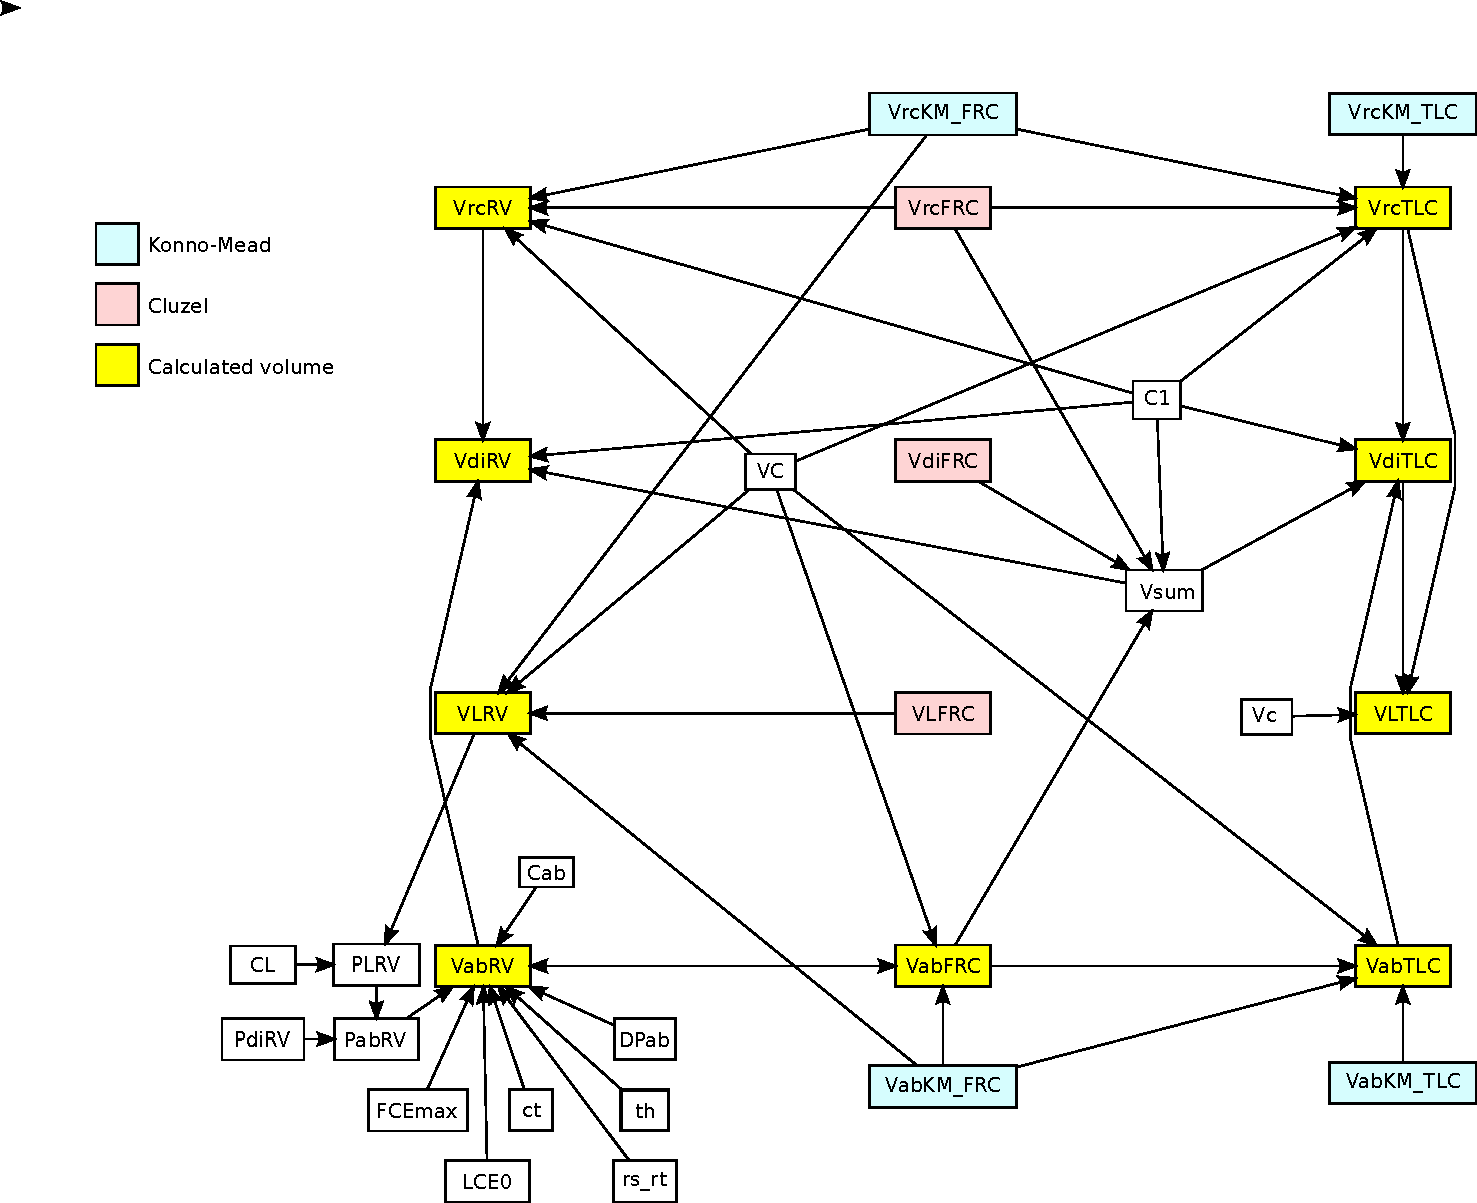
\includegraphics[width=6in]{paramgen.pdf}

\nohyphens{
\bibliographystyle{apalike}
\bibliography{references}
%\printbibliography{references}
}
\printindex

\end{document}
